% input files

% document's head
% \phantom{42}

\begin{center}
    \LARGE \textsc{Заметки курса <<Электричество и магнетизм>>}
\end{center}

\hrule

\phantom{42}

\begin{flushright}
    \begin{tabular}{rr}
    % written by:
        \textbf{Автор}: 
        & Хоружий Кирилл \\
        &\\
    % date:
        \textbf{От}: &
        \textit{\today}\\
    \end{tabular}
\end{flushright}

\thispagestyle{empty}
\tableofcontents
% \newpage

%%%%%%%%%%%%%%%%%%%%%%%%%%%%%%%%%%%%%%%%%%%%%%%%%%%%%%%%%%%%%%%%%%%%%%%%%%%%%%%%%%%
\section*{Свёртка и приближение функций бесконечно гладкими}
\setcounter{section}{1}
\addcontentsline{toc}{section}{Свёртка и приближение функций бесконечно гладкими}
%%%%%%%%%%%%%%%%%%%%%%%%%%%%%%%%%%%%%%%%%%%%%%%%%%%%%%%%%%%%%%%%%%%%%%%%%%%%%%%%%%%

\sbsnum{1}{Свёртка функций и её свойства}
Для точки $P$ движущейся относительно некоторого неподвижного тела (свяжем с ним точку $O$), можно ввести следующие характеристики:
\begin{to_def}[Радиус вектор, скорость и ускорение точки $P$]
	\begin{equation*}
	\vc{r} = \overrightarrow{O P},
	\hspace*{1 cm}
	\vc{v} = \frac{d \vc{r}}{d \vc{t}},
	\hspace*{1 cm}
	\vc{w} =  \frac{d \vc{v}}{d t} = \frac{d^2 \vc{r}}{d t^2}.
\end{equation*}	
\end{to_def}

\begin{to_def}
	Для задания движения точки, зная её траекторию, можно сопоставить ей дуговую координату $\sigma (t)$ и получить выражения для скорости и ускорения, выраженные в осях \textit{естественного трёхгранника} $\vc{\tau}, \vc{n}, \vc{b}$.
	Таким образом для $\vc{r} = \vc{r}(\sigma(t))$:
	\begin{equation*}
		\vc{\tau} (\sigma) = \frac{d \vc{r}}{d \sigma}, 
		\hspace*{1 cm} 
		\frac{d \vc{\tau}}{d \sigma} = \frac{1}{\rho} \vc{n} (\sigma),
	\end{equation*}
	где $\rho$ -- радиус кривизны. Для кривой в $\mathbb{R}^3$ добавим ещё вектор $b$ для правой тройки. Таким образом получим формулы Френе:
	\begin{equation*}
		\frac{d \vc{\tau}}{d s} = \frac{1}{\rho} \vc{n},
		\hspace*{1 cm}
		\frac{d \vc{n}}{d s} = - \frac{1}{\rho} \vc{\tau} + \varkappa \vc{b},
		\hspace*{1 cm}
		\frac{d \vc{b}}{d s} = - \varkappa \vc{n}.
	\end{equation*}
\end{to_def}

Таким образом сможем в компонентах трёхгранника выписать скорость и ускорение точки:
\begin{gather*}
   \vc{v} = \frac{d \vc{r}}{d t} = \frac{d \vc{r}}{d \sigma} \frac{d \sigma}{d t} = v_\tau \vc{\tau}
   \\
   \vc{w} = \frac{d \vc{v}}{d t} = \frac{d_\tau}{d t} \vc{\tau} + v_\tau \frac{d \vc{\tau}}{d \sigma} \frac{d \sigma}{d t} = \frac{d^2 \sigma}{d t^2} \vc{\tau} + \frac{v_\tau^2}{\rho} \vc{n}.
\end{gather*}
Как видно, ускорение точки представилось в видео $w = w_n + w_\tau $ --- \textit{нормальной} и \textit{тангенциальной} составляющей.

\begin{to_lem}[Из матана]
	Для $f_i \in  C^2 \colon U \mapsto V$, если $X$ -- касательный вектор в точке $p \in U$, то $X(f)$ можно определить как:
	\begin{equation*}
		X(f) = X(x^i) \frac{\partial f(p)}{\partial x^i}, \text{ а координаты этого вектора в криволинейных координатах: } X = X^i \frac{\partial}{\partial x^i}.
	\end{equation*}
\end{to_lem}

Каждую материальную точку можем определить $\vc{r}_1, \ldots, \vc{r}_N$ -- итого $\mathbb{R}^{3N}$. Но есть некоторые ограничения вида
\begin{equation*}
    f_i (\vc{r}, t) = 0.
\end{equation*}
Вложим в фазовое пространство многообразие $M$, в котором локально всё хорошо. Тогда
$\dim M = n$ -- число степеней свободы, а параметризация $q_1, \ldots, q_N$ -- криволинейные координаты. В каждой $A \in M$ верно, что $\dot{\vc{q}} \in TM_A$, то есть
\begin{equation*}
    TM = \bigcup_q T_qM \ni (q, \dot{q})
\end{equation*}

И так, движение точки можно задать, если её криволинейные координаты --- известне функции $q(t)$.
\begin{equation*}
	\vc{r} = \vc{r}(q_1, q_2, q_3) = x \vc{i} + y \vc{j} + z \vc{k}.
\end{equation*}

\begin{to_def}
	\textit{Коэффициентами Ламе} такие $H^i$. C их помощью удобно выразить единичные базисные векторы криволинейных координат: 
	\begin{equation*}
		H_i = \left|\frac{\partial \vc{r}}{\partial q^i} \right| = \sqrt{\left(\frac{\partial x}{\partial q^i}\right)^2 + \left(\frac{\partial y}{\partial q^i}\right)^2 + \left(\frac{\partial z}{\partial q^i}\right)^2}.
		\hspace*{1 cm}
		e^i = \frac{1}{H_i} \frac{\partial \vc{r}}{\partial q^i}.
	\end{equation*}
\end{to_def}

Далее будем координатными векторами называть $\vc{g}_i(\vc{r}) = \frac{\partial \vc{r}}{\partial q^i}$. Разложение произвольного вектора по локальному базису имеет вид:
\begin{equation*}
	\vc{a} = a^i \vc{g}_i = a_j \vc{g}^j.
\end{equation*}
Здесь $\vc{g}^j$ --- векторы двойственного базиса к базису из $\vc{g}_i$. В двойственном же (взаимном) базисе из матана мы видели:
\begin{equation*}
	X(f) = d f (X) = \partial_x f,
	\hspace*{1 cm}
	d x^i (\frac{\partial}{\partial x^j}) = \frac{\partial x^i}{\partial x^j} = \delta_j^i,
	\hspace*{1 cm}
	a = a_i d x^i.
\end{equation*}
Таким образом получаем скорость точки и её ковариантную компоненту:
\begin{equation*}
	\vc{v} = \frac{d \vc{r}}{d t} = \frac{\partial \vc{r}}{\partial q^i} \frac{d q^i}{d t} = \vc{g}_i \dot{q}^i,
	\hspace*{1 cm}
	v^i = \vc{q}^i.
\end{equation*}
И для ускорения:
\begin{equation*}
	w_k = \left(\frac{d \vc{v}}{d t}\right)_k = \frac{(d \vc{v})_k}{d t} = g_{k j} \frac{d v^j}{d t} + \Gamma_{k i j} v^j v^i.
\end{equation*}


\sbsnum{2}{Бесконечно гладкие функции с компактным носителем}
\begin{proof}[\ref{lem_6.20}]
	
	1) для введённой $\varphi$ достаточно: $\varphi_\varepsilon (x_1,\ldots,x_n) = A \varphi\left(\frac{\sqrt{n} x_1}{\varepsilon}\right)\ldots\varphi\left(\frac{\sqrt{n} x_n}{\varepsilon}\right)$.

	2) $\psi(x) = B \int_{-\infty}^x \varphi(t) \d t $, выбирем $B$: $\psi(x) \equiv 0 \; \forall x \leq 1$ и $\psi(x) \equiv 1 \; \forall x \geq -1$;

	3) достаточно положить: $\psi_{\varepsilon,\delta} (x) = \psi \left(\frac{\delta +\varepsilon -2|x|}{\varepsilon-\delta}\right)$.
\end{proof}

\sbsnum{3}{Приближение функций бесконечно гладкими}
\begin{proof}[\ref{thr_6.21}]
	
	1) $f_k(x) - f(x) = \int_{\mathbb{R}^n} (f(x-t) - f(x)) \varphi_k(t) \d t$;

	2) Пусть $f$ р-но непр. в $U_\delta(K\subset \mathbb{R}^n) $ и пусть $|f(x) - f(y)|<\varepsilon$ при $|x-y|<\delta$ там же;

	3) Выбирая $k\colon 1/k <\delta$, тогда $\varphi_k(t) \neq 0 $ при $|t|<\delta$ и тогда $|f(x-t) - f(x)|<\varepsilon$ при $x \in K$.

	4) при $x \in K$ верна р-ная сходимость: $|f_k(x) - f(x)| \leq \varepsilon \int_{\mathbb{R}^n}\varphi_k(x) \d x = \varepsilon$.

	5) продифференцируем по параметру $\int_{\mathbb{R}^n} f(t) \varphi_k (x-t)\d t $;

	6) производная (5) при $x \in K$ будет зависеть только значений $f$ в $U_{1/k}(K)$, то есть $f$ можно считать интегрируемой при дифференцировании по параметру, что позволяет применять теорему.
\end{proof}

\begin{proof}[\ref{thr_6.22}]
	 По различным $\partial_{x_i} f*\varphi_k(x)$ получим по лемме \ref{lem_6.19}, для производных свёрток схожее равенство, с самой $f$, а значит и р-ную сходимость.
	\begin{equation*}
		\frac{\partial^m (f*\varphi_k)}{\partial x_{i_1}\ldots \partial x_{i_m}} = \frac{\partial^m f}{\partial x_{i_1}\ldots \partial x_{i_m}}*\varphi_k.
	\end{equation*}
\end{proof}

\begin{proof}[\ref{thr_6.23}]
	1) по thr(\ref{thr_5.75}) $f = h + g$, где $g$ -- эл. ступ., $\int_{\mathbb{R}^n} |h|\d x <\varepsilon$;

	2) по thr(\ref{thr_6.18}): $\int_{\mathbb{R}^n}|h * \varphi_k|\d x < \varepsilon$. То есть, если окажется: $\int_{\mathbb{R}^n}|g - g*`f_k|\d x < \varepsilon$, то
	\begin{equation*}
		\int_{\mathbb{R}^n}|f - f*\varphi_k| \d x \leq \int_{\mathbb{R}^n} |g - g* \varphi_k|\d x + \int_{\mathbb{R}^n}|h|\d x + \int_{\mathbb{R}^n} |h*\varphi_k| \d x < 3 \varepsilon.
	\end{equation*}

	3) Раскладывая $g$ в сумму х-их $\chi_P$, останется доказать для одной $\chi_P$;

	4) $\chi_P - \chi_P - \varphi_k \neq 0$ только в $U_{1/k}(\partial P) $ и по модулю $\leq 1$;

	5) То есть после интегрирования получим не более $\mu(U_{1/k}(\partial P))$.

	6) Напрямую можно убедиться, что эта $\mu \mapsto 0$ при $k\mapsto 0$.
\end{proof}

\newpage

%%%%%%%%%%%%%%%%%%%%%%%%%%%%%%%%%%%%%%%%%%%%%%%%%%%%%%%%%%%%%%%%%%%%%%%%%%%%%%%%%%%
\section*{Дифференцируемые отображения и криволинейные замены координат}
\setcounter{section}{2}
\addcontentsline{toc}{section}{Дифференцируемые отображения и криволинейные замены координат}
%%%%%%%%%%%%%%%%%%%%%%%%%%%%%%%%%%%%%%%%%%%%%%%%%%%%%%%%%%%%%%%%%%%%%%%%%%%%%%%%%%%

\sbsnum{4}{Дифференцируемые отображения и дифференцирование композиции}
\subsubsection*{Теорема о сложении скоростей}
\begin{to_thr}
	Абсолютная скорость точки равна сумме переносной и относительной скорости: $\vc{v}^a = \vc{v}^e + \vc{v}^r$.
\end{to_thr}
\begin{proof}[$\triangle$]
	Для точки $P$ в абсолютной системе координат:
	\begin{equation*}
		\vc{R} = \vc{R}_0 + \vc{r}
		\hspace*{1 cm}
		\Rightarrow
		\hspace*{1 cm}
		\vc{v}_a = \vc{\dot{R}} = \vc{\dot{R}}_0 + \vc{\dot{r}} = \underbrace{\vc{v}_0 + \vc{\omega}\times \vc{r}}_{v^e} + \underbrace{A \vc{\dot{\rho}}}_{v^r}.
	\end{equation*}
	\textit{Переносная скорость} $v^e$ --- есть скорость той точки подвижной системы координат, в которой находится $P$.
	Таким образом показали напрямую разложение.
\end{proof}

\subsubsection*{Теорема Кориолиса}
\begin{to_thr}
	Абсолютное ускорение точки равно сумме переносного, относительного и карелысого ускорения: $w^a = w^e + w^r + w^c$.
\end{to_thr}
\begin{proof}[$\triangle$]
	Для абсолютного ускорения точки, продифференцируем ещё раз:
	\begin{equation*}
		\vc{w}^a = \vc{\dot{v}}_0 + \vc{\dot{\omega}} \times \vc{\dot{r}} + \vc{\omega} \times \vc{\dot{r}} + \dot{A} \vc{\dot{\rho}} + A \vc{\ddot{\rho}} = w_0 + \vc{\varepsilon} \times \vc{r} + \vc{\omega} \times (\vc{\omega} \times \vc{r} + A \vc{\dot{\rho}}) + \dot{A} \vc{\dot{\rho}} + A \vc{\ddot{\rho}}.
	\end{equation*}
	$\vc{\varepsilon}$ --- угловое ускорение подвижной системы координат, а $A \ddot{\rho} = w^r$:
	\begin{equation*}
		w^a = \underbrace{ w_0 + \vc{\varepsilon} \times \vc{r} + \vc{\omega} \times (\vc{\omega} \times \vc{r})}_{w^e} + w^r + \omega \times A \vc{\dot{\rho}} + \dot{A} \vc{\dot{\rho}}.
	\end{equation*}
	И последние два слогаемых дадут кареолисового ускорение: $\dot{A} \vc{\dot{\rho}} = \dot{A} A^{-1} A \vc{\dot{\rho}} = \vc{\omega} \times A \vc{\dot{\rho}} $, тогда получаем $w^c = 2 \vc{\omega} \times v^r$. Итого получаем искомую формулу.
\end{proof}


\sbsnum{5}{Системы криволинейных координат и теорема об обратном отображении}
% 6.4. Непрерывно дифференцируемые отображения и криволинейные системы координат

\begin{to_def} 
    \textit{Криволинейная замена координат} --- бесконечно гладкое отображение $\varphi \colon U \to V$ такое, что $\varphi^{-1}$ определено и тоже бесконечно гладко. 
\end{to_def}

\begin{to_lem} 
    Пусть открытое множество $U \subset \mathbb{R}^n $ выпукло. Для непрерывно дифференцируемого отображения $\varphi \colon U \to \mathbb{R}^m $ найдётся непрерывное отображение $A \colon U \times U \to \mathcal L (\mathbb{R}^n, \mathbb{R}^m)$, такое что $\forall x', \ x'' \in U$ 
\begin{equation*}
     \varphi(x'') - \varphi(x') = A(x', x'')(x'' - x')
 \end{equation*} 
 и $A(x, x) = D \varphi_x$.  
\end{to_lem}

% \begin{to_lem} 
%     Для всякого линейного отображения $A \colon \mathbb{R}^n \mapsto \mathbb{R}^m$ найдётся число $\|A\|$ такое что для все $x \in \mathbb{R}^n$ $|Ax| \leq \|A\| \cdot |x|$. 
% \end{to_lem}

\begin{to_thr}[Теорема об обратном отображении]
     \textbf{Если} отображение $\varphi \colon U \mapsto \mathbb{R}^n$ непрерывно дифференцируемо в окрестности точки $x$ \textbf{и} его дифференциал $D\varphi_x$ являетсяя невырожденным линейным преобразованием, \textbf{то} это отображение взаимно однозначно отображает некоторую окрестность $V \ni x$ на окрестность $W \ni y$, где $y = \varphi(x)$. Обратное отображение $\varphi^{-1} \colon W \to V$ тоже непрерывно дифференцируемо. 
\end{to_thr}


\begin{to_def} 
    \textit{Криволинейной системой координат} в окрестности точки $p \in \mathbb{R}^n$ называется набор таких функций, которые явяются координатами гладкого отображения окрестности $p$ на некоторое открытое множество в $\mathbb{R}^n$ с гладким обратным\footnote{
        По теореме об обратном отображении для проверки системы преобразования достаточно проверить невырожденность $\left(
    \partial y_i / \partial x_j
    \right)$ в точке $p$, или линейную независимость $dy^i$ в точке $p$.
    } отображением.
\end{to_def}



\sbsnum{6}{Теоремы о системе неявных функций}
\begin{to_thr}[Теорема о неявной функции]
\label{thr_6.32}
     Пусть функции $f_1, \ldots, f_k$ непрерывно дифференцируемы в окрестности $p \in \mathbb{R}^n$ и 
    \begin{equation*}
        \det \left(
            \frac{\partial f_i}{\partial x_j} 
        \right) \neq 0
    \end{equation*}
    в этой окрестности. Пусть $f_i(p) = y_i$, $i = 1, \ldots, k$. Тогда найдётся окрестность точки $p$ вида $U \times V$, $U \subset \mathbb{R}^k$, $V \subset \mathbb{R}^{n-k}$, такая что в этой окрестности множество решений системы уравнений
    \begin{equation*}
        \left\{\begin{aligned}
            f_1(x) &= y_1, \\
            &\ldots \\
            f_k(x) &= y_k,
        \end{aligned}\right.
    \end{equation*}
    совпадает с графиком непрерывно дифференцируемого отображения $\varphi \colon V \to U$, заданного в координатах как
    \begin{equation*}
        \left\{\begin{aligned}
            x_1 &= \varphi_1 (y_1, \ldots, y_k,\ x_{k+1}, \ldots, x_n),\\
            &\ldots\\
            x_k &= \varphi_k (y_1, \ldots, y_k,\ x_{k+1}, \ldots, x_n),
        \end{aligned}\right.
    \end{equation*}
    то есть отображения $\mathbb{R}^{n-k} \mapsto \mathbb{R}^k$.
\end{to_thr}


\sbsnum{7}{Теорема о расщеплении гладкого отображения}
\subsubsection*{Свободные и несвободные системы. Связи.}

В общем случае связь запишем, как
$$
    f(\vc{r}_\nu, \vc{v}_\nu, t) \geq 0.
$$
В частности, при $f(\vc{r}_\nu, \vc{v}_\nu, t) = 0$, связь называет \textit{двухсторонней}, или \textit{удерживающей}. При неравенстве, соотвественно, связь \textit{односторонняя}, \textit{освобождающая}.
Связь вида $f(\vc{r}_\nu, t) = 0$ называется \textit{геометрической}, \textit{конечная}, \textit{голономная}. Связь вида $f(\vc{r}_\nu, \vc{v}_\nu, t) = 0$ называется \textit{дифференциальной}, или \textit{кинематической}. Иногда кинематическая связь может быть представлена как геометрическая, такая связь называется \textit{интегрируемой}. 

\begin{to_def} 
     Если на систему материальных точек не наложены дифференциальные неинтегрируемые связи, то она называется голономной. Если же среди связей, наложенных на систему есть дифференциальные неинтегрируемые связи, то система называется неголономной.
\end{to_def}

Хотелось бы построить некоторую общую теорию для случая, когда этих связей несколько. 
В частности пусть есть $r$ геометрических связей.
\begin{equation}
\label{eqs1}
    f_\alpha (\vc{r}, t) = 0, \hspace{0.5cm} (\alpha = 1, \ldots, r),
\end{equation}
И несколько дифференциальных линейных связей
\begin{equation}
\label{eqs2}
    \sum_{\nu=1}^N \vc{a}_{\beta \nu} (\vc{r}_1, \ldots, \vc{r}_N, t) \cdot \vc{v}_\nu + a_\beta  (\vc{r}_1, \ldots, \vc{r}_N, t) = 0,
    \hspace{0.5cm} (\beta = 1, \ldots, s)
\end{equation}
Стоит сказать, что число \textit{степеней} \textit{свободы} данной системы:
$$
    3N - r - s \geq 1.
$$

\begin{to_def} 
     Геометрические связи называются стационарными или склерономными, если $t$ не входит в их уравнения \eqref{eqs1}. Дифференциальные связи \eqref{eqs2} называются \textit{стационарными} или \textit{склерономными} если функции $\vc{a}_{\beta\nu}$ не зависят явно от $t$, а функции $a_\beta \equiv 0$. Система называется \textit{склерономной}, если она либо свободная, либо на нее наложены только стационарные связи. Система называется \textit{реономной}, если среди наложенных на нее связей есть хотя бы одна нестационарная.
\end{to_def}

\subsubsection*{Ограничения, налагаемые связями на положения, скорости, ускорения и перемещения точек системы.}

Пусть задан некоторый момент $t = t*$. Тогда \textit{возможными положениями} назовём $\vc{r}_\nu$ такие, что для них верно \eqref{eqs1}, \eqref{eqs2}. 

Какие возможны скорости?
\begin{equation}
    \label{eqs3}
    \sum_{\nu=1}^N \frac{\partial f_\alpha}{\partial \vc{r}_\nu} \cdot \vc{v}_\nu +   \frac{\partial f_\alpha}{\partial t} = 0, \hspace{0.5cm} (\alpha = 1, \ldots, r).
\end{equation}

Совокупность векторов $\vc{v}_\nu = \vc{v}_\nu^*$, удовлетворяющая линейным
уравнениям \eqref{eqs2} и \eqref{eqs3} в возможном для данного момента времени положении
системы, назовем возможными скоростями. 

Какие возможны ускорения?
\begin{align}
\label{eqs4}
    \eqref{eqs3}, \eqref{eqs2}
    \hspace{0.25cm} \overset{d / dt}{\Rightarrow} \hspace{0.25cm} 
    & \sum_{\nu=1}^N \frac{\partial f_\alpha}{\partial \vc{r}_\nu} \cdot \vc{\mathrm{w}}_\nu +
    \sum_{\nu, \mu=1}^N \frac{\partial^2 f_\alpha}{\partial \vc{r}_\nu \partial \vc{r}_\mu} \vc{v}_\mu \cdot \vc{v}_\nu + 2 \sum_{k=1}^N \frac{\partial^2 f_\alpha}{\partial t \partial \vc{r}_\nu} \vc{v}_\nu + \frac{\partial^2 f_\alpha}{\partial t^2}  = 0 
    \hspace{0.25cm} &\alpha \in [1, r]\\
\label{eqs5}
    & \sum_{\nu=1}^N \vc{a}_{\beta\nu} \cdot \vc{\mathrm{w}}_\nu + \sum_{\nu, \mu =1}^N \frac{\partial \vc{a}_{\beta\nu}}{\partial \vc{r}_\mu} \vc{v}_\mu \cdot \vc{v}_\nu + \sum_{\nu=1}^N \frac{\partial \vc{a}_{\beta\nu}}{\partial t} \cdot \vc{v}_\nu + \sum_{\nu=1}^N \frac{\partial a_\beta}{\partial \vc{r}_\nu} \cdot \vc{v}_\nu + \frac{\partial  a_\beta}{\partial t} = 0
     \hspace{0.25cm} &\beta \in [1, s]
\end{align}

Совокупность векторов $\vc{\mathrm{w}}_\nu =\vc{\mathrm{w}}_\nu^*$, удовлетворяющая линейным
уравнениям \eqref{eqs4} и \eqref{eqs5} в возможном для данного момента времени положении
системы (+скорости), назовем возможными скоростями. 

Рассмотрим возможные перемещения $\Delta \vc{r}_\nu$ системы за $\Delta t$ из её возможного положения $\vc{r}_\nu^*$ в момент $t=t^*$. Тогда 
\begin{equation}
    \Delta \vc{r}_\nu = \vc{v}^* \Delta t + \frac{1}{2} \vc{\mathrm{w}}_\nu^* (\Delta t)^2 + \ldots
    \hspace{0.5cm} (\nu = 1, \ldots, N).
\end{equation}
Пренебрегая нелинейными членами, получим, что $\Delta \vc{r}_\nu = \vc{v}_\nu^* \Delta t$. Тогда, домножив \eqref{eqs2}, \eqref{eqs3} на $\Delta t$, получим систему уравнений, которой удовлетворяют линейные по $\Delta t$ возможные перемещения:
\begin{align}
\label{eqs7}
    \sum_{\nu=1}^N \frac{\partial f_\alpha}{\partial \vc{r}_\nu} \cdot \Delta \vc{r}_\nu + \frac{\partial f_\alpha}{\partial t} \Delta t &= 0,
    \hspace{0.5cm} &(\alpha = 1, \ldots, r), \\
\label{eqs8}
    \sum_{\nu=1}^N \vc{a}_{\beta\nu} \cdot \Delta \vc{r}_\nu + a_\beta \Delta t &= 0,
    \hspace{0.5cm} &(\beta = 1, \ldots, s),
\end{align}
где функции $\vc{a}_{\beta\nu}, a_\beta$ и частные производные вычисляются при $t=t^*, \; \vc{r}_\nu = \vc{r}_\nu^*$.


\subsubsection*{Действительные и виртуальные перемещения}
Пусть задано положение системы для $t, \vc{r}, \vc{v}, \vc{\mathrm{w}}$. Тогда для $t = t^* + dt$ запишем, что
\begin{equation}
\label{eqs9}
    \vc{r}_\nu (t^* + dt) - \vc{r}_\nu (t^*) = \vc{v}_{\nu_0}^* \d t + \frac{1}{2} \vc{\mathrm{w}}^*_{\nu_0} (dt)^2 + \ldots,
\end{equation}
где $\vc{\mathrm{w}}_{\nu_0}^*$ -- ускорения точек системы при $t = t^*$. Величины \eqref{eqs9} -- \textit{действительные (истинные) перемещения} точек системы за время $dt$. Тогда получим систему уравнений, аналогичную \eqref{eqs7}, \eqref{eqs8}:
\begin{align}
\label{eqs10}
    \sum_{\nu=1}^N \frac{\partial f_\alpha}{\partial \vc{r}_\nu} \cdot d \vc{r}_\nu + \frac{\partial f_\alpha}{\partial t} d t &= 0,
    \hspace{0.5cm} &(\alpha = 1, \ldots, r), \\
\label{eqs11}
    \sum_{\nu=1}^N \vc{a}_{\beta\nu} \cdot d \vc{r}_\nu + a_\beta d t &= 0,
    \hspace{0.5cm} &(\beta = 1, \ldots, s).
\end{align}


Помимо действительных перемещений есть \textit{виртуальные}. Ими называется совокупность величин $\delta \vc{r}_\nu$, удовлетворяющая линейным однородным уравнениям
\begin{align}
\label{eqs12}
    \sum_{\nu=1}^N \frac{\partial f_\alpha}{\partial \vc{r}_\nu} \cdot \delta \vc{r}_\nu  &= 0,
    \hspace{0.5cm} &(\alpha = 1, \ldots, r), \\
\label{eqs13}
    \sum_{\nu=1}^N \vc{a}_{\beta\nu} \cdot \delta \vc{r}_\nu  &= 0,
    \hspace{0.5cm} &(\beta = 1, \ldots, s),
\end{align}
Если система склерономна, то действительное перемещение будет одним из виртуальных.

\begin{to_def} 
    \textit{Синхронное варьирование} -- переход из одного положения в другое, при фиксированном времени
    $$
        \vc{r}_\nu^* \to \vc{r}_\nu^* + \delta \vc{r}_\nu.
    $$
    При синхронном варьировании мы не рассматриваем процесс движения и сравниваем допускаемые связями
    бесконечно близкие положения (конфигурации) системы для данного фиксированного момента времени.
\end{to_def}

Рассмотрим две совокупности возможных перемещений с одним и тем же значением величины $\Delta t$. Согласно разложению по Тейлору,
\begin{align*}
    \Delta_1 \vc{r}_\nu = \vc{v}_{\nu_1}^* \Delta t + \frac{1}{2} \vc{\mathrm{w}}_{\nu_1}^* (\Delta t)^2 + \ldots, \\
    \Delta_2 \vc{r}_\nu = \vc{v}_{\nu_2}^* \Delta t + \frac{1}{2} \vc{\mathrm{w}}_{\nu_2}^* (\Delta t)^2 + \ldots, 
\end{align*}
и рассмотрим их разность
$$
        \Delta_1 \vc{r}_\nu - \Delta_2 \vc{r}_\nu = (\vc{v}_{\nu_1}^* \Delta t - \vc{v}_{\nu_2}^* \Delta t) + \left(\frac{1}{2} \vc{\mathrm{w}}_{\nu_1}^* (\Delta t)^2 - \frac{1}{2} \vc{\mathrm{w}}_{\nu_2}^* (\Delta t)^2\right) + \ldots.
$$

\subsubsection*{Идеальные связи}
\begin{to_def}
	Связи называют \textit{идеальными}, если сумма работ этих связей на любых виртуальных перемещениях всегда равна нулю: $\sum \vc{R}_\nu \delta \vc{r}_\nu = 0$.
\end{to_def}

Абсолютно твердое тело является системой материальных точек, в которой на любые две точки наложена идеальная связь. При отсутствии других других связей, кроме между точками тела, твердое тело называют \textit{свободным}.

Считая связи идеальными запишем уравнения для материальных точек системы:
\begin{equation*}
	m_{\nu} \vc{w}_\nu = \vc{F}_\nu + \vc{R}_\nu
	\hspace*{0.3 cm}
	\Rightarrow
	\hspace*{0.3 cm}
	\left(
	\sum_{\nu=1}^N \vc{R}_\nu \delta \vc{r}_\nu = 0\right)
	\hspace*{0.3 cm}
	\Rightarrow
	\hspace*{0.3 cm}
	\sum_{\nu = 1}^{N}(\vc{F}_\nu - m_\nu \vc{w}_\nu) \delta \vc{r}_{\nu} = 0.
\end{equation*}
Последнее равенство называется общим уравнением динамики. Оно выполняется всегда для любого совместимого со связям движения, соответствующего заданным активным силам $\vc{F}{\nu}$.

Если же наоборот, дано какое-то совместимое со связями движение системы, для которого выполняется общее уравнение динамики, тогда с $\vc{R}_\nu = m_\nu \vc{w}_\nu - \vc{F}_\nu$ будем иметь равенства для задания уравнений несвободной системы. Мы считаем, что эти силы реакции реализуются в действительности и что рассматриваемое движение соответствует активным силам $\vc{F}_\nu (t,r_\nu, v_\nu)$.

Таким образом  \textit{общее уравнение динамики выражает необходимое и достаточное условие того, чтобы движение, совместимое со связями, соответствовало заданной системе активных сил}.

Взяв выражения для виртуальных перемещений всегда можно получить силы реакции так называемым методом \textit{множителей Лагранжа}:
\begin{equation*}
	\sum_{\nu=1}^N \left(\vc{R}_\nu - \sum_{i = 1}^d \lambda_i \frac{\partial f_i}{\partial \vc{r}_\nu} - \sum_{j = 1}^s \mu_j \alpha_{j \nu}\right) \delta \vc{r}_\nu = 0
	\hspace*{1 cm}
	\Rightarrow
	\hspace*{1 cm}
	\vc{R}_\nu = \sum_{i = 1}^d \lambda_i \frac{\partial f_i}{\partial \vc{r}_\nu} + \sum_{j = 1}^s \mu_j \alpha_{j \nu}.
\end{equation*}
Полученные выражения для реакций идеальных сил через неопределенные множители Лагранжа $\lambda_i $ и $\mu_j $ можно подставить в исходное уравнение связей, получим \textit{уравнения Лагранжа первого рода}:
\begin{equation*}
	m_\nu \vc{w}_\nu = \vc{F}_\nu + \sum_{i = 1}^d \lambda_i \frac{\partial f_i}{\partial \vc{r}_\nu} + \sum_{j = 1}^s \mu_j \alpha_{j \nu}.
\end{equation*}

\newpage

%%%%%%%%%%%%%%%%%%%%%%%%%%%%%%%%%%%%%%%%%%%%%%%%%%%%%%%%%%%%%%%%%%%%%%%%%%%%%%%%%%%
\section*{Дифференциал, гессиан, и исследование функции на экстремум}
\setcounter{section}{3}
\addcontentsline{toc}{section}{Дифференциал, гессиан, и исследование функции на экстремум}
%%%%%%%%%%%%%%%%%%%%%%%%%%%%%%%%%%%%%%%%%%%%%%%%%%%%%%%%%%%%%%%%%%%%%%%%%%%%%%%%%%%

\sbsnum{9}{Локальные экстремумы функции и необходимое условие экстремума}
\begin{to_def}
	Точка $p$ называется локальным экстремумом функции $f$, если она является точкой экстремума (максимума или минимума) ограничения $f$ на некоторую окрестность $p$.
	\label{def_6.36}
\end{to_def}

\begin{to_thr}[Необходимое условие экстремума]
	\begin{equation*}
		\left\{\begin{aligned}
	    	&f \in C^1(U(p))\\
	    	&p \text{ --- def(\ref{def_6.36})}
		\end{aligned} \right.
		\hspace*{0.5 cm} \Rightarrow \hspace*{0.5 cm}
		\d f_p = 0.
	\end{equation*}
	\label{thr_6.37}
\end{to_thr}



\sbsnum{10}{Необходимые и достаточные условия экстремума
 \texorpdfstring{$\text{C}^2$}{C2}  функций}
\begin{to_thr}[Необходимые условия экстремума]
	\begin{equation*}
	\left\{\begin{aligned}
	    	&f \in C^2(U(p))\\
	    	&p \text{ --- def(\ref{def_6.36})} \\
	    	& \d f_p = 0
		\end{aligned} \right.
		\hspace*{0.5 cm} 
		\Rightarrow
		 \hspace*{0.5 cm}
		\left[
		\begin{aligned}
			\d_2 f_p \geq 0 \text{ --- min}\\
			\d_2 f_p \leq 0	\text{ --- max}
		\end{aligned}\right.
\end{equation*}	
\end{to_thr}

\begin{to_lem}
	Если квадратичная форма $Q > 0$, \textbf{то} $\exists \varepsilon>0 \colon $ $Q(v) \geq \varepsilon|v|^2 \;(\forall v)$.
	\label{lem_6.38}
\end{to_lem}


\begin{to_thr}[Достаточные условия экстремума]
\begin{equation*}
	\left\{\begin{aligned}
	    	&f \in C^2(U(p))\\
	    	&p \text{ --- def(\ref{def_6.36})}\\
	    	&\d f_p = 0 \text{ и } \d_2 f_p <0 
		\end{aligned} \right.
	\hspace*{0.5 cm} 
	 \Rightarrow
	  \hspace*{0.5 cm}
	p \text{ --- точка строгого локального максимума}
	\label{thr_6.39}
\end{equation*}
\end{to_thr}

\sbsnum{11}{Условные экстремумы и необходимое условие в терминах первых производных}
\begin{to_def}
	Условный экстремум f --- экстремум ограничения $f$ на множество $S$, задаваемое системой $C^1$ уравнений $\varphi_1(x) = \ldots = \varphi_m(x) = 0$.

	Забегая вперёд, нам самом деле нам нужно: $\dim \langle \d \varphi_1, \ldots, \d \varphi_m\rangle = m$.
	\label{def_usl_ext}
\end{to_def}

\begin{to_thr}[Необходимые условия условного экстремума в терминах первых произ-водных]
	 \begin{equation*}
	 \left\{
	 	\begin{aligned}
	 		&f, \varphi_1,\ldots,\varphi_m \in C^1(U(p))\\
	 		&\dim \langle \d \varphi_1, \ldots, \d \varphi_m\rangle = m\\
	 		&p \text{ --- def(\ref{def_usl_ext})}
	 	\end{aligned}\right.
	 	\hspace*{0.5 cm} \Rightarrow \hspace*{0.5 cm}
	 	\d f_p = \lambda_1 \d \varphi_{1,p} + \ldots + \lambda_m \d \varphi_{m,p}.
	 \end{equation*}
	 \label{thr_6.42}
\end{to_thr}


\sbsnum{12}{Необходимые и достаточные условия в терминах вторых производных}
Удобно положить: $L(x) = f(x) - \lambda_1 \varphi_1(x) - \ldots - \lambda_m \varphi_m(x)$. Это называется \textit{функцией Лагранжа},а $\lambda_{i}$ --- \textit{множители Лагранжа}.

\begin{to_thr}[Необходимые условия условного экстремума]
	\begin{equation*}
	 \left\{
	 	\begin{aligned}
	 		&f, \varphi_1,\ldots,\varphi_m \in C^2(U(p))\\
	 		&\dim \langle \d \varphi_1, \ldots, \d \varphi_m\rangle = m\\
	 		&p \text{ --- def(\ref{def_usl_ext})}\\
	 		&\vc{v}\colon \d \varphi_{1,p}(\vc{v}) = \ldots = \d \varphi_{m,p}(\vc{v}) = 0
	 	\end{aligned}\right.
	 	\hspace*{0.5 cm} \Rightarrow \hspace*{0.5 cm}
	 	\left\{
	 	\begin{aligned}
	 		&\d L_p = 0\\
	 		&\left[
	 		\begin{aligned}
	 			&\d_2 L_p \geq 0 (\text{для минимума})\\
	 			&\d_2 L_p \leq 0 (\text{для максимума})
	 		\end{aligned}\right.
	 	\end{aligned}\right.
	 \end{equation*}
	 \label{thr_6.42}
\end{to_thr}

\begin{to_thr}[Достаточные условия условного экстремума]
	\begin{equation*}
		\left\{
		\begin{aligned}
	 		&f, \varphi_1,\ldots,\varphi_m \in C^2(U(p))\\
	 		&\dim \langle \d \varphi_1, \ldots, \d \varphi_m\rangle = m\\
	 		&\d L_p = 0\\
	 		&\varphi_1(p) = \ldots = \varphi_m(p) = 0\\
	 		&\vc{v}(\neq 0) \colon \d \varphi_{1,p}(\vc{v}) = \ldots = \d \varphi_{m,p}(\vc{v}) = 0\\
	 		&\d_2 L(\vc{v}) > 0 \text{ или } \d_2 L(\vc{v}) < 0
	 	\end{aligned}\right.
	 	\hspace*{0.5 cm} \Rightarrow \hspace*{0.5 cm}
	 	f \text{ имеет строгий условный экстремум в } p.
	\end{equation*}
	\label{thr_6.43}
\end{to_thr}

\newpage

%%%%%%%%%%%%%%%%%%%%%%%%%%%%%%%%%%%%%%%%%%%%%%%%%%%%%%%%%%%%%%%%%%%%%%%%%%%%%%%%%%%
\section*{Векторы и дифференциальные формы первой степени}
\setcounter{section}{4}
\addcontentsline{toc}{section}{Векторы и дифференциальны формы первой степени}
%%%%%%%%%%%%%%%%%%%%%%%%%%%%%%%%%%%%%%%%%%%%%%%%%%%%%%%%%%%%%%%%%%%%%%%%%%%%%%%%%%%

\sbsnum{13}{Вектор, как дифференцирование}


% 6.6. Векторы и векторные поля

\begin{to_lem} 
    \label{lem_6.44}
    Всякую гладкую функцию, определенную в некоторой окрестности $x_0 \in \mathbb{R}^n$, в возможно меньшей окрестности $x_0$, можно представить в виде
    \begin{equation*}
         f(x) = f(x_0) + \sum_{k=1}^n \partial_k f|_{x_0}
         \
         (x^k  - x_0^k) , 
     \end{equation*} 
     с гладкими $\partial_k f$.
\end{to_lem}

% Начнём наше удивительное приключение в определение вектора. Для всякого $v \in \mathbb{R}^n$ мы можем определеить производную по направлению
% \begin{equation*}
%     \frac{\partial f}{\partial v}  = \lim_{t \to 0} 
%     \left(
%         \frac{f(p+tv)-f(p)}{t} 
%     \right),
%     \hspace{0.5cm} 
%     \frac{\partial (fg)}{\partial v} = \frac{\partial f}{\partial v} g + f \frac{\partial g}{\partial v}.
% \end{equation*}
% Проблема -- $p + tv$ определено не инвариантно. Решение -- определим вектор, как \textit{дифференцирование алгебры гладких функций в точке}, удовлетворяющее формуле Лейбница.

\begin{to_def} 
    Определим \textit{касательный вектор} в точке $p \in U$ открытого множества $U \subseteq \mathbb{R}^n$ как $\mathbb{R}$-линейное отоборражение $X \colon C^{\infty}(U) \mapsto \mathbb{R}$, удовлетворяющее 
    \begin{equation*}
        X(fg) = X(f) g(p) + f(p) X(g).
    \end{equation*}
    \textit{Касательное пространство} $T_p U$ к $U$ в точке $p$ состоит из всех касательных векторов в точке $p$.
\end{to_def}

\begin{to_lem} 
    Если $X$ -- касательный вектор в точке $p \in U$, то для любой окресности $V \ni p$, $V \subseteq U$, выражение $X(f)$ может зависеть только от значений $f$ в $V$, а не на всём $U$. 
\end{to_lem}

В силу предыдущих лем мы можем перейти в окрестность, где $f$ представима в виде \eqref{lem_6.44}, тогда
\begin{equation*}
    X(f) = X(f(p)) + \sum_{i=1}^n X(x_i) \partial_i f|_p + \sum_{i=1}^n x_i(p) X(\partial_i f|_p) = 
    \sum_{i=1}^n X(x_i) \ \partial_i f|_p.
\end{equation*}
Числа $X_i = X(x_i)$ называются координатами касательного вектора в данной криволинейной системе координат, тогда весь вектор в точке $p$ записывается, как $X = X^i \partial_i$.


\sbsnum{14}{Касательное пространство и дифференциал отображения}

\begin{to_def} 
    \textit{Векторным полем} на открытом множестве $U \subseteq \mathbb{R}^n$ называется выбор касательного вектора $X(p) \in T_p U$ для каждой точки $p \in U$, гладко\footnote{
        Гладкая зависимость понимается в смысле гладкой зависимости координат векторного поля $X_i(p)$ в точке $p$.
    } зависящий от $p$.  
\end{to_def}


\begin{to_lem} 
    Для открытого $U \subseteq \mathbb{R}^n$ всякое $\mathbb{R}$-линейное отображение $X \colon C^{\infty} \mapsto C^{\infty}(U)$, удовлетворяющее правилу Лейбница $X(fg) = X(f) g + f x(g)$ задаётся векторным полем на $U$. 
\end{to_lem}



\begin{to_def} 
    Пусть есть вектор $X \in T_pU,$ $q = \varphi(p)$, тогда \textit{прямой\footnote{
        Производную отображения $\varphi$ в точке $p$ можно определить как $\varphi_*\colon T_p U \mapsto  T_q V$ при $q = \varphi(p)$. Иначе можем обозначать, как $F \varphi_p$.
    } образ вектора} $\varphi_*(X)$ определяется по формуле
    \begin{equation*}
        \varphi_* (X) f = X(f \circ \varphi),
        \hspace{1cm}\mapsto\  \left(\varphi_*X\right)^i = \frac{\partial \varphi^i}{\partial x^j} X^j 
        \hspace{0.25cm} \Leftrightarrow \hspace{0.25cm} 
        \text{\red{переписать в матричном виде}}
        .
    \end{equation*}
\end{to_def}

\begin{to_def} 
    Отображение $\varphi \colon U \mapsto  V$ задаёт \textit{гомоморфизм алгебр} (операция, сохраняющая умножение, сложение, и переводящая $\const$ в $\const$): 
    $\varphi^* \colon C^{\infty}(V) \mapsto C^{\infty}(U)$ по формуле
    \begin{equation*}
        \varphi^* (f) = f \circ \varphi.
    \end{equation*}
    вектор даёт дифференцирование алгебры $X \colon C^{\infty}(U) \mapsto \mathbb{R}$, и тогда $\varphi_* X = X \circ \varphi^*$ тоже дифференцирование алгебры. 
\end{to_def}



\sbsnum{15}{Диф-формы I степени}
\subsubsection*{Метод комплексных амплитуд}


Рассмтрим $U = U_0 \cos (\Omega t + \varphi)$. По методу комплексных амплитуд
\begin{equation*}
    U = U_0 e^{i\left(\Omega t + \varphi \right)}.
\end{equation*}
Он применим всегда, когда $\Re$ и $\Im$ не смешиваются. 

Можем ввести импеданс -- комплексное сопротивление, при чём $\Re(z)$ -- активное сопротивление, $\Im z$ -- реактивное споротивление. 

\subsubsection*{Мощность переменного тока}
Рассмотрим некоторый элемент
\begin{equation*}
    I = I_0 \cos \left(\Omega t + \psi\right) = \Re I_0 e^{i \psi} e^{i \Omega t}, \hspace{0.5cm} 
    U = U_0 \cos (\Omega t + \varphi) = \Re U_0 e^{i\varphi} e^{i \Omega t}.
\end{equation*}
Мгновенное значение мощности
\begin{equation*}
    P = UI = 
    \frac{1}{2} I_0 U_0 \cos (\psi - \varphi) + \frac{1}{2} I_0 U_0 \cos (
    2 \Omega t + \varphi + \psi
    ),
    \hspace{0.5cm} \Rightarrow \hspace{0.5cm} 
    \langle P\rangle_T = \frac{1}{T} \int P \d t = \frac{1}{2} I_0 U_0 \cos (\psi - \varphi).
\end{equation*}
Можно исправить метод комплексных амплитуд сопряжением.
\begin{equation*}
    \langle P\rangle_T = \frac{1}{2} \tilde I \tilde U^*,
    \hspace{0.5cm} 
    I_{\text{эфф}} = \frac{1}{T} \int_0^T I^2 \d t = \frac{I_0}{\sqrt{2}},
    \hspace{0.5cm} 
    U_{\text{эфф}} = \frac{1}{T} \int_0^T U^2 \d t.
\end{equation*}


 

\newpage 

%%%%%%%%%%%%%%%%%%%%%%%%%%%%%%%%%%%%%%%%%%%%%%%%%%%%%%%%%%%%%%%%%%%%%%%%%%%%%%%%%%%
\section*{Диф-формы высших степеней}
\setcounter{section}{5}
\addcontentsline{toc}{section}{Диф-формы высших степеней}
%%%%%%%%%%%%%%%%%%%%%%%%%%%%%%%%%%%%%%%%%%%%%%%%%%%%%%%%%%%%%%%%%%%%%%%%%%%%%%%%%%%

\sbsnum{16}{Определение и свойства диф-форм высших степеней}
\begin{to_def} 
    Определим \textit{дифференциальную форму степени} $k$ на открытом $U \subseteq \mathbb{R}^n$ как кососимметричное отображение наборов из $k$ гладких векторных полей $X_1, \ldots, X_k$ на $U$ в $C^{\infty}(U)$, линейное по каждому аргументу и относительно умножения на бесконечно гладкие функции.
\end{to_def}

\begin{to_lem} 
    Значение выражения $\alpha(X_1, \ldots, X_k)$ в точке $p$ зависит только от значений векторных полей $X_i$ в точке $p$.     
\end{to_lem}

Пространство диф-форм степени $k$ на $U \subseteq \mathbb{R}^n$ обозначим $\Omega^k(U)$. Интересно, что $\Omega^n(U)$ в фиксированной системе координат выглядит как $C^{\infty}(U)$, но при замене координат ведёт себя иначе.

% Для $ \forall f \in C^{\infty}(U)$ её дифференциал, как отображение $U \mapsto \mathbb{R}$ можно считать формой первой степени $df(X) = X(f)$. 


\red{Свойства диф-форм?}






\sbsnum{17}{Внешнее умножение диф-форм}
\begin{to_def} 
    \textit{Внешнее умножение} $\Omega^k(U) \times \Omega^l (U) \mapsto \Omega^{k+l} (U)$, можно определить как $\alpha \wedge \beta = \text{Alt}\, (\alpha \otimes \beta)$, где
    \begin{equation*}
        \text{Alt}\, (T(\ldots)) = \frac{1}{(k+l)!} \sum_{\sigma \in \Sigma_{k+l}} \sign \sigma \cdot T(\sigma(\ldots)),
    \end{equation*}
    при чём $(dx_1 \wedge \ldots \wedge dx_k)(\partial_1, \ldots, \partial_k) = 1$.
\end{to_def}



\sbsnum{18}{Внешнее дифференцирование}
\begin{to_lem} 
    На гладких диф-формах на $U$ существует единсвтенный $\mathbb{R}$-линейный оператор $d \colon \Omega^k (U) \mapsto \Omega^{k+1} (U)$, удовлетворяющий условиям: 
    1) $d(f) = df$;
    2) $d^2 = 0$;
    3) $d(\alpha \wedge \beta) = d \alpha \wedge \beta + (-1)^{\deg \alpha} \alpha \wedge d \beta$ (а-ля правило Лейбница).
    Более того, операция $d$ определена инвариантно.
\end{to_lem}


\begin{to_def} 
    Внешнему дифференцированию 0,1,2-форм в ориентированном $\mathbb{R}^3$ отвечают соответственнооперации \textit{градиента} скалярного поля, \textit{ротора} и \textit{дивергенции} векторного поля, определнные соотношениями
\begin{equation*}
     d \omega^0_f \overset{\mathrm{def}}{=} \omega^1_{\grad f}, \hspace{1cm} 
     d \omega^1_{\vv{A}} \overset{\mathrm{def}}{=} \omega^2_{\rot \vv{A}}, \hspace{1cm} 
     d \omega^2_{\vv{B}} \overset{\mathrm{def}}{=} \omega^3_{\div \vv{B}}.
 \end{equation*} 
    Также можно определить $\Delta \vc{A}$, как
\begin{equation*}
    \Delta \vc{A} = \grad \div \vc{A} - \rot \rot A.
\end{equation*}
\end{to_def}







\sbsnum{19}{Обратный образ диф-форм}
\begin{equation*}
    \alpha + \frac{\alpha}{\beta} 
\end{equation*}


\newpage 


%%%%%%%%%%%%%%%%%%%%%%%%%%%%%%%%%%%%%%%%%%%%%%%%%%%%%%%%%%%%%%%%%%%%%%%%%%%%%%%%%%%
\section*{Интегрирование дифференциальных форм}
\setcounter{section}{6}
\addcontentsline{toc}{section}{Интегрирование дифференциальных форм}
%%%%%%%%%%%%%%%%%%%%%%%%%%%%%%%%%%%%%%%%%%%%%%%%%%%%%%%%%%%%%%%%%%%%%%%%%%%%%%%%%%%

\sbsnum{20}{Интегрирование диф-формы объёма}
Естественно ввести \textit{тензор электромагнитного поля}:
\begin{equation}
{F}_{ik} = 
    \begin{pmatrix}
        0    & E_x & E_y  & E_z   \\
        -E_x  & 0    & -B_z & B_y   \\
        -E_y & B_z  & 0    & -B_x  \\
        -E_z & -B_y & B_x & 0     \\
    \end{pmatrix}_{ik},
    \hspace{2cm} 
{F}^{ik} = 
    \begin{pmatrix}
        0    & -E_x & -E_y  & -E_z   \\
        E_x  & 0    & -B_z & B_y   \\
        E_y & B_z  & 0    & -B_x  \\
        E_z & -B_y & B_x & 0     \\
    \end{pmatrix}^{ik}
\end{equation}
Тогда уравнения Максвелла запишутся в виде
\begin{equation}
    \boxed{
        \varepsilon^{iklm} \partial_k F_{lm} = 0, \hspace{0.5cm} 
        \partial_k F^{ik} = - \frac{4\pi}{c} j^i
    },
\end{equation}
где $j^i = (\rho c, \vc{j})$. Прямой подстановкой тензора ЭМ поля нетрудно убедиться, что

\phantom{42}

\noindent
\begin{minipage}[t]{0.45\textwidth}
\noindent
Дифференциальная форма в СГС:
    \begin{align}
        \vphantom{\oint }
        \div \vc{D} &= 4 \pi \rho \\
        \vphantom{\oint }
        \div \vc{B} &= 0 \\
        \vphantom{\oint }
        \rot \vc{E} &= -\frac{1}{c} \frac{\partial \vc{B}}{\partial t}  \\
        \vphantom{\oint }
        \rot \vc{H} &= \frac{4\pi}{c} \vc{j} + \frac{1}{c} \frac{\partial \vc{D}}{\partial t} 
    \end{align}
\end{minipage}
\hfill
\begin{minipage}[t]{0.45\textwidth}
Интегральная форма в СГС:
    \begin{align}
       \oint \vc{D} \cdot d \vc{s} &= 4\pi Q \\
       \oint \vc{B} \cdot d \vc{s} &= 0 \\
       \oint \vc{E} \cdot d \vc{l} &= - \frac{1}{c} \frac{d}{dt} \int \vc{B} \cdot d \vc{s} \\
        \oint \vc{H} \cdot \d \vc{l} &= \frac{4\pi}{c} I + \frac{1}{c} \frac{d}{dt} \int \vc{D} \cdot \d \vc{s}.
    \end{align}
\end{minipage}

\begin{description*}
    \item[$\vc{E}$]  --- напряженность электрического поля;
    \item[$\vc{H}$]  --- напряженность магнитного поля;
    \item[$\vc{D}$]  --- электрическая индукция;
    \item[$\vc{B}$]  --- магнитная индукция.
\end{description*}

\subsubsection*{Материальные уравнения}

В проводниках связь между плотностью тока и напряжённостью электрического поля выражается в линейном приближении \textit{законом Ома}:
\begin{equation*}
    \vc{j} = \sigma \vc{E},
\end{equation*}
где $\sigma$ -- \textit{удельная проводимость среды}.

В среде сторонние электрические и магнитные поля вызывают поляризация $\vc{P}$ и намагничивание вещества $\vc{M}$.
Тогда
\begin{align*}
    \rho_\text{b} &= - \nabla \cdot \vc{P} \\
    \vc{j}_\text{b} &= c \nabla \times \vc{M} + \frac{\partial \vc{P}}{\partial t} ,
\end{align*}
Далее, по определению
\begin{align*}
    \vc{D} &= \vc{E} + 4\pi \vc{P}, &\vc{B} &= \vc{H} + 4 \pi \vc{M} \\
\end{align*}
Что в случае линейной поляризации или линейной намагничиваемости можно записать, как  
$$
    \left\{\begin{aligned}
        \vc{P} &= \chi_{\text{e}} \vc{E}, \\
        \vc{M} &= \chi_{\text{m}} \vc{H}, \\
    \end{aligned}\right.
    \hspace{0.5cm} \Rightarrow \hspace{0.5cm} 
    \left\{\begin{aligned}
         \vc{D} &= \varepsilon \vc{E} = (1 + 4\pi \chi_{\text{e}}) \vc{E}, \\
       \vc{B} &= \mu \vc{H} = (1 + 4 \pi \chi_{\text{m}}) \vc{H}.
    \end{aligned}\right.
$$
где $\varepsilon$ -- \textit{\cancel{относительная} диэлектрическая проницаемость}, $\mu$  — \textit{относительная магнитная проницаемость}, $\chi_{\text{e}}$  -- \textit{диэлектрическая восприимчивость}, $\chi_{\text{m}}$ -- \textit{магнитная восприимчивость}.

Наконец, в однородных средах верно, что
\begin{equation*}
    \left\{\begin{aligned}
        \div \vc{E} &= 4\pi \frac{\rho}{\varepsilon},  \\
        \div \vc{B} &= 0,
    \end{aligned}\right.
    \hspace{1cm} 
    \left\{\begin{aligned}
        \rot \vc{E} &= - \frac{1}{c} \frac{\partial \vc{B}}{\partial t}, \\
        \rot \vc{B} &= \frac{4\pi}{c} \mu \vc{j} + \frac{\varepsilon \mu}{c} \frac{\partial \vc{E}}{\partial t},
    \end{aligned}\right.
\end{equation*}
где в оптическом диапазоне принято $n = \sqrt{\varepsilon \mu}$.

\subsubsection*{Граничные условия}
Опять же, в СГС,
\begin{equation*}
    \left\{\begin{aligned}
        (\vc{E}_1 - \vc{E}_2) \times \vc{n}_{1,2} &= 0, \\
        (\vc{H}_1 - \vc{H}_2) \times \vc{n}_{1,2} &= \frac{4\pi}{c} \vc{j}_\text{s},
    \end{aligned}\right.
    \hspace{1cm} 
    \left\{\begin{aligned}
        \left(\vc{D}_1 - \vc{D}_2\right) \cdot \vc{n}_{1,2} &= - 4\pi \rho_\text{s}, \\
        \left(\vc{B}_1 - \vc{B}_2\right) \cdot \vc{n}_{1, 2} &= 0,
    \end{aligned}\right.
\end{equation*}
где $\rho_{\text{s}}$ -- поверхностная плотность свободных зарядов, $\vc{j}_\text{s}$ -- плотность поверхностных свободных токов вдоль границы. 

Эти граничные условия показывают непрерывность нормальной компоненты вектора магнитной индукции, и непрерывность на границе областей тангенциальных компонент напряжённостей электрического поля. 

\subsubsection*{Уравнение непрерывности}

Источники полей $\rho, \vc{j}$ не могут быть заданы произвольным образом. Применяя операцию дивергенции к четвёртому уравнению (закон Ампера—Максвелла) и используя первое уравнение (закон Гаусса), получаем уравнение непрерывности
\begin{equation*}
    \nabla \cdot \vc{j} + \frac{\partial \rho}{\partial t} = 0,
    \hspace{0.5cm} \Leftrightarrow \hspace{0.5cm} 
    \oint_S \vc{j} \cdot \d \vc{s} = - \frac{d }{d t} \int_V \rho \d V.
\end{equation*}




\sbsnum{21}{Представление диф-формы в каноническом виде}
Вспомнив пару уравнений Максвелла и домножив на $\vc{H}, \ \vc{E}$ соответственно, получим
\begin{equation*}
    \left\{\begin{aligned}
        \rot \vc{E} &= - \frac{1}{c} \frac{\partial \vc{H}}{\partial t}, \\
        \rot \vc{H} &= \frac{1}{c} \frac{\partial \vc{E}}{\partial t} + \frac{4\pi}{c} \vc{j}
    \end{aligned}\right.
    \hspace{0.5cm} \Rightarrow \hspace{0.5cm} 
    \frac{1}{c} \vc{E} \frac{\partial \vc{E}}{\partial t} + 
    \frac{4\pi}{c} \vc{E} \cdot \vc{j} + 
    \frac{1}{c} \vc{H} \frac{\partial \vc{H}}{\partial t} =
    \underbrace{
        \vc{E} \rot \vc{H} - \vc{H} \rot \vc{E}
    }_{
        -\div \left[ \vc{E} \times \vc{H} \right]
    }.
\end{equation*}
Поэтому естественно ввести следующее определение:
\begin{equation}
    \vc{S} = \frac{c}{4\pi} \left[\vc{E} \times \vc{H} \right]
    \text{\ \ --- \textit{вектор Умова-Пойтинга}}.
\end{equation}
Тогда уравнение перепишется в следующем виде (теорема Пойтинга в диф-форме):
\begin{equation}
    \frac{\partial }{\partial t} \frac{E^2 + H^2}{8\pi} = - \vc{E} \cdot \vc{j} - \div \vc{S}.
\end{equation}
Проинтегрировав по некоторому объему, поймём, что
\begin{equation}
    \frac{\partial }{\partial t} \int \frac{E^2 + H^2}{8\pi} \d V = 
    - \int \vc{j} \cdot \vc{E} \d V -
    \oint \vc{S} \cdot \d \vc{f},
\end{equation}
вспомнив скорость изменения кинетической энергии, получим, так называемую, \textit{теорему Пойтинга}
\begin{equation}
    \begin{aligned}
        e \vc{E} \cdot \vc{v} = \frac{d }{d t} \mathcal E_{\text{кин}}, \\
        \int \vc{j} \cdot \vc{E} \d V = \sum e \vc{v} \cdot \vc{E},
    \end{aligned}
    \hspace{0.5cm} \longrightarrow \hspace{0.5cm} 
    \frac{\partial }{\partial t} 
    \left[
        \int \frac{E^2 + H^2}{8\pi} \d V + \sum \mathcal{E}_{\text{кин}}
    \right] = 
    - \oint_{\partial V} \vc{S} \cdot \d \vc{f}.
\end{equation}
И теперь уже естественно разделить левую часть на энергию зарядов, и энергию поля:
\begin{equation*}
    \mathcal{W} = \frac{E^2 + H^2}{8\pi} 
    \text{\ \ --- \textit{плотность энергии} ЭМ поля},
\end{equation*}
а также ввести следующую величину:
\begin{equation*}
    \oint_{\partial V} \vc{S} \cdot \d \vc{f} 
    \text{\ \ --- \textit{поток энергии}  ЭМ поля}.
\end{equation*}

\sbsnum{22}{Поведение интеграла от формы при линейной замене координат}

\begin{to_lem}[Поведение интеграла формы при линейной замене координат]
     Интеграл дифференциальной формы $\nu \in \Omega_{\text{c}}^n (\mathbb{R}^n)$ при отображении $A^*$, соответствующем линейному преобразованию $A : \mathbb{R}^n \mapsto  \mathbb{R}^n$ меняет или не меняет знак в зависимости от знака определителя $\det A$, то есть
     \begin{equation*}
         \int_{\mathbb{R}^n} A^* \nu = (\sign \det A) \int_{\mathbb{R}^n} \nu.
     \end{equation*}
\end{to_lem}


\sbsnum{23}{Гладкое разбиение единицы}
Пусть каждой точке среды соответсвует $\xi^1, \xi^2, \xi^3$, собственно $(\xi, t)$ -- \textit{лгранжевы переменные}. \textit{Закон движения среды} в таком случае это
\begin{equation}
    \vc{r} (\xi, t),
\end{equation}
скорость же
$$
    \vc{v} = \frac{\partial \vc{r}(\xi, t)}{\partial t},
    \hspace{0.5cm} 
    \vc{\mathrm{w}} = \frac{\partial \vc{v} (\xi, t)}{\partial t},
$$
и так далее.

Альтернативно можеем задать $(x, t)$ -- эйлерово описание. Тогда
$$
    \vc{v}(x, t), \vc{\mathrm{w}}(x, t) 
    \hspace{0.5cm} \text{-- поля скоростей и ускорений.}
$$

В частности, представляя движение по шоссе, полоса 1,2,3 и участок трассы -- эйлерово описание среды.
Если же мы будем следить за каждой машиной, то это будет лагранжево описание.

\sbsnum{24}{Поведение интеграла от формы при гладкой замене координат}
Длинная линия — модель линии передачи, продольный размер (длина) которой превышает длину волны, распространяющейся в ней. Такая линия передачи может быть охаракетризована погонными параметрами:
$R_0$ -- погонное сопротивление, $G_0$ -- паразитная, погонная проводимость, $L_0$ -- погонная индуктивность, $C_0$ -- погонная емкость.


Рассмотрим два рядом идущих длинных провода (коаксиальный кабель, например). Тогда в $z$ и $z+ \Delta z$ ток будет различным, как и, соответсвенно, разность потенцаилов. 
\begin{equation*}
    V(z+\Delta z) - V(z) = \frac{L_0 \Delta z}{c^2} \frac{\partial I}{\partial t},
    \hspace{1cm} 
    I(z) = I(z+\Delta z) + \frac{\partial q}{\partial t},
    \hspace{1cm} 
    q = C_0 \Delta z V.
\end{equation*}

\begin{figure}[h]
    \centering
    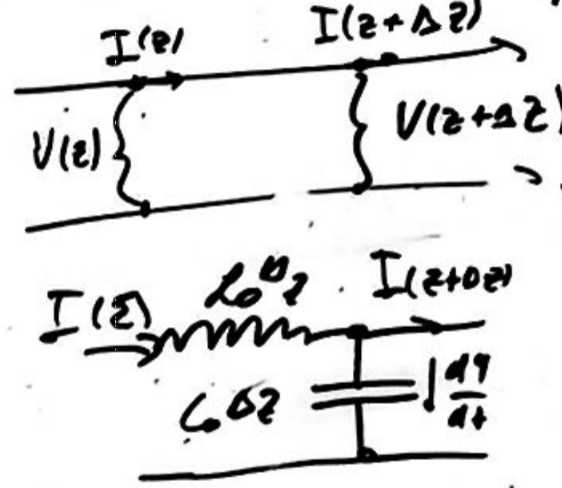
\includegraphics[width=0.25\textwidth]{img/2.png}
    %\caption{}
    %\label{fig:}
\end{figure}

\noindent
Из этих уравнений легко получить, что
\begin{equation}
    \left\{\begin{aligned}
        \frac{\partial U}{\partial z} &= - \frac{L_0}{c^2} \frac{d I}{d t} \\
        \frac{\partial I}{\partial z} &= - C_0 \frac{\partial U}{\partial t} 
    \end{aligned}\right.
    \hspace{0.5cm} \Rightarrow \hspace{0.5cm} 
    \boxed{
        \frac{\partial^2 U}{\partial t^2}  = \frac{c^2}{L_0 C_0} - \frac{\partial^2 V}{\partial z^2} 
    }.
\end{equation}
Решение аналогично будем искать в виде
\begin{equation}
    V = f_1 (z - vt) + f_2 (z + vt),
    \hspace{0.5cm} \Rightarrow \hspace{0.5cm} 
    v = \frac{c}{\sqrt{L_0 C_0}}.
\end{equation}
Кстати, если это всё посчитать для коаксиального кабеля, то
\begin{equation*}
    L_0 = 2 \mu \ln \frac{R_2}{R_1} , \hspace{0.5cm} 
    C_0 = \frac{\varepsilon}{2 \ln \frac{R_2}{R_1} },
    \hspace{0.5cm} \Rightarrow \hspace{0.5cm} 
    v = \frac{c}{\sqrt{\mu \varepsilon}}.
\end{equation*}


\subsubsection*{Коэффициент стоячей волны (standing wave ratio)}
Коэффициент стоячей волны -- отношение наибольшего значения амплитуды напряжённости электрического или магнитного поля стоячей волны в пучностях линии передачи к амплитуде в узлах.
КСВ является мерой согласования нагрузки (например, антенны) с линией передачи.

Наибольшее и наименьшее значения амплитуды соответсвенно равны
\begin{equation*}
    A_{\text{max}} = A_{\text{inc}} + A_{\text{ref}}, \hspace{0.5cm} 
    A_{\text{min}} = A_{\text{inc}} - A_{\text{ref}},
    \hspace{0.5cm} \Rightarrow \hspace{0.5cm} 
    \text{КСВ} = \frac{A_{\text{inc}} + A_{\text{ref}}}{A_{\text{inc}} - A_{\text{ref}}} = 
    \frac{1 + |\Gamma|}{1 - |\Gamma|},
\end{equation*}
где $|\Gamma|$ -- коэффициент отражения.

\subsubsection*{Согласованная нагрузка}
Рассмотрим длинную линию, пусть в цепи 
\begin{equation*}
    U = U_0 \cos \left(\omega_0 t - kz\right),  \hspace{0.5cm} 
    I = I_0 \cos \left(\omega_0 t - kz\right).
\end{equation*}
Сделаем следующий трюк. Возьмем, и продолжим линию до бесконечности, от которой, очевидно, ничего не отразится. Соотвественно нас интересует поиск эквивалентного импеданса системы. 
\begin{align*}
    U^* = U_0 \exp\left(i(\omega_0 t - kz)\right) &= U_0 e^{ikz} e^{-i\omega_0 t}, \\
    I^* = I_0 \exp\left(i(\omega_0 t - kz)\right) &= I_0 e^{ikz} e^{-i\omega_0 t}.
\end{align*}
Подставив эти выражения в волновое уравнение, и получим
\begin{equation*}
    ik U^* = i \omega_0 I^*,
    \hspace{0.5cm} 
    Z^* = U^* / I^* = \frac{\omega_0}{k},
    \hspace{0.5cm} \Rightarrow \hspace{0.5cm} 
    R = \frac{1}{c} \sqrt{\frac{L_0}{C_0}},
    \text{\ \ --- \ \ \textit{согласованная нагрузка}}.
\end{equation*}
То есть при наличии такого сопротивления на конце линии не будет никакого отражения. 




\sbsnum{25}{Формулы гладкой замены переменных в интеграле Лебега от функции}
\subsubsection*{Уравнение непрерывности}
\begin{to_def}[Предмет рассмотрения]
	Ввиду макроскопического рассмотрения \textit{жидкости}(газы) в гидродинамике представлется как сплошная среда, то есть малый элемент объёма жидкости содержит ещё достаточно больше количество молекул, относительно межмолекулярного расстояния.
\end{to_def}

Для описания движения жидкости требуется задать распределение скорости жидкости $\vc{v} = \vc{v}(x,y,z,t)$ и какие-либо её две термодинамические величины, как, например, плотность и давление. Важно отметить, что все эти величины относятся не к отдельной частице, а к точке в пространстве в определенное время.

\begin{to_thr}[Уравнение непрерывности]
\phantom{239}

\begin{proof}[$\triangle$]
	В маленьком объёме $V_{0}$ количество жидкости есть $\int_{V_0} \rho d V$.
	Через элемент поверхности, ограничивающей $V_0$, в единицу времени протекает $\rho \vc{v} \cdot d \vc{f}$ жидкости --- положительно или отрицательное число, в зависимости от того, вытекает или втекает жидкость соответственно.
	Тогда приравниваем для вытекания жидкости два наших рассуждения:
	\begin{equation*}
		- \frac{\partial}{\partial t} \int \rho d V =  \oint \rho \vc{v} \cdot d \vc{f}
		\hspace*{0.5 cm} 
		\Rightarrow 
		\hspace*{0.5 cm}
		\int \left(\frac{\partial \rho}{\partial t} + \div \rho \vc{v}\right)d V = 0
		\hspace*{0.5 cm}
		\Rightarrow
		\hspace*{0.5 cm}
		\frac{\partial \rho}{\partial t} + \div \rho \vc{v} = 0.
	\end{equation*}
	Последнее следует из того, что равенство должно иметь для любого объёма, таким образом получили искомое \textit{уравнение непрерывности}.
\end{proof}
	
\end{to_thr}

\subsubsection*{Уравнение Эйлера}

\begin{to_thr}[Уравнение Эйлера]
\phantom{239}

\begin{proof}[$\triangle$]
	Выделим в жидкости некоторый объём, полная сила, действующая на этот объём: $- \oint p d \vc{f} = - \int \grad p d V$, где интеграл из взятого по поверхности объёма преобразуется в сам рассматриваемый объём.
	Таким образом получили, что на единицу объёма жидкости будет действовать сила:
	\begin{equation*}
		\rho \frac{d \vc{v}}{d t} = - \grad p.
	\end{equation*}
	Однако стоящая здесь скорость определяет изменение скорости именно элемента объёма, а не точки в пространстве.
	Запишем это изменение скорости:
	\begin{equation*}
		d \vc{v} 
		=
		 \frac{\partial \vc{v}}{\partial t} d t + \frac{\partial \vc{v}}{\partial x^i} d x^i 
		= 
		\frac{\partial \vc{v}}{\partial t} d t + (d \vc{r} \cdot \nabla) \vc{v}
		\hspace*{1 cm}
		\Rightarrow
		\hspace*{1 cm}
		\frac{\partial \vc{v}}{\partial t} + (\vc{v} \nabla) \vc{v} = - \frac{1}{\rho} \grad p.
	\end{equation*}
	Последнее и есть искомое уравнение Эйлера.
\end{proof}
\end{to_thr}

Если же жидкость движется во внешнем поле тяжести, то, на каждый элемент объёма будет действовать сила, которая просто добавится к изначальному уравнению: 
\begin{equation*}
	\frac{\partial \vc{v}}{\partial t} + (\vc{v} \nabla) \vc{v} = - \frac{\nabla p}{\rho} + \vc{g}.
\end{equation*}

\subsubsection*{Уравнение Навье-Стокса}

Чтобы нормально учесть вязкость, нужно поговорить про \textit{поток импульса}.
Импульс единицы объёма жидкости есть $\rho \vc{v}$, скорость изменения его компоненты:
\begin{equation*}
	\frac{\partial}{\partial t} \rho v^i = \rho \frac{\partial v^i}{\partial t} + \frac{\partial \rho}{\partial t} v^i.
\end{equation*}
Уравнения непрерывности и Эйлера запишутся в тензорном виде:
\begin{equation*}
	\frac{\partial \rho}{\partial t} = - \frac{\partial (\rho v^k)}{\partial x^k},
	\hspace*{0.5 cm}
	\hspace*{0.5 cm}
	\frac{\partial v^i}{\partial t} = - v^k \frac{\partial v^i}{\partial x^k} - \frac{1}{\rho} \delta^{i k} \frac{\partial p}{\partial x^k}.
\end{equation*}
Тогда получим:
\begin{equation*}
	\frac{\partial}{\partial t} \rho v^i 
	= 
	- \rho v^k \frac{\partial v^i}{\partial x^k} -  \delta^{i k} \frac{\partial p}{\partial x^k} - v^i \frac{\partial \rho v^k}{\partial x^k} 
	=
	-\delta^{i k} \frac{\partial p}{\partial x^k} - \frac{\partial}{\partial x^k} \rho v^i v^k
	= - \frac{\partial \Pi^{i k}}{\partial x^k}.
\end{equation*}
\begin{to_def}
	$\Pi^{i k} $ --- \textit{тензор плотности потока импульса}:
	$
		\Pi^{i k} = p \delta^{i k} + \rho v^i v^k.
	$
\end{to_def}

Таким образом уравнение Эйлера у нас записалось в виде:
$
	\frac{\partial}{\partial t} \rho v^i = - \frac{\partial \Pi^{i k}}{\partial x^k}.
$
Поток импульса представляет собой чисто обратимый перенос импульса, связанный с просто механическим передвижением различных участков жидкости и с действующими в жидкости силами давления.
\textit{Вязкость} (внутреннее трение) жидкости проявляется в наличии ещё дополнительного, необратимого переноса импульса из мест с большой скоростью в места с меньшей.

Поэтому уравнение движения вязкой жидкости можно получить, прибавив к идеальному потоку импульса дополнительный член $\sigma^{i k}_{visc}$, определяющий такой вязкий перенос:
$
\Pi^{i k} = p \delta^{i k} + \rho v^i v^k - \sigma^{i k}_{visc} = - \sigma^{i k} + \rho v^i v^k.
$
\begin{to_def}
	Таким образом: $\sigma^{i k} = - p \delta^{i k} + \sigma^{i k}_{visc}$ называют \textit{тензором напряжений}, а $\sigma^{i k}_{visc}$ --- вязким тензором напряжений.
\end{to_def}

Чтобы написать выражение для вязкого напряжения сделаем пару оговорок. 
\textit{Во первых}, градиенты скорости движения участков жидкости относительно друг друга не велики, тогда $\sigma^{i k}_{visc}$ зависит лишь от первых производных скорости по координатам, линейно. \textit{Во вторых}, не зависящие от первых производных величины должны обращаться в нуль как для скорости потока $\vc{v} = \const$ и тензор должен быть нулевым. \textit{В третьих}, $\sigma^{i k}_{visc} = 0$ когда жидкость совершает целое равномерное вращение, поскольку никакого внутреннего трения тогда не будет.
Для такого равномерного вращения с $\vc{v} = [\vc{\omega} \vc{r}]$ линейными комбинациями производных обращающимися в нуль будут: $\frac{\partial v^i}{\partial x^k} + \frac{\partial v^k}{\partial x^i}$.

Это всё даёт нам мотивацию для не шибко сильных потоков несжимаемой жидкости согласится с Сэром Исааком Ньютоном, и написать тензор вязкого напряжения, как \textit{тензор скорости деформации}:
\begin{equation*}
	\sigma^{i k}_{visc} = \eta \left(\frac{\partial v^i}{\partial x^k} + \frac{\partial v^k}{\partial x^i}\right),
	\hspace*{1 cm}
	\Rightarrow
	\hspace*{1 cm}
	\sigma^{i k} = - p \delta^{i k} + \eta \left(\frac{\partial v^i}{\partial x^k} + \frac{\partial v^k}{\partial x^i}\right).
\end{equation*}
А уравнение Эйлера тогда для несжимаемой жидкости запишется:
\begin{equation*}
	\rho \left(\frac{\partial v^i}{\partial t} + v^k \frac{\partial v^i}{\partial x^k}\right)
	=
	- \delta^{i k} \frac{\partial p}{\partial x^k} + \frac{\partial}{\partial x^k} \left[\eta \left(\frac{\partial v^i}{\partial x^k} + \frac{\partial v^k}{\partial x^i}\right)\right].
\end{equation*}
а в более человеческом, привычном глазу, виде \textit{уравнение Навье-Стокса для несжимаемой жидкости}:
\begin{equation*}
	\frac{\partial \vc{v}}{\partial t} + (\vc{v} \triangle) \vc{v} = - \frac{1}{\rho} \grad p + \frac{\eta}{\rho} \Delta \vc{v}.
\end{equation*}
\begin{to_def}
	Коэффициент $\eta$ называется --- \textit{динамическим коэффициентом вязкости}, а отношение $\eta/\rho = \nu$ --- \textit{кинематической вязкостью}.
\end{to_def}


\newpage 


%%%%%%%%%%%%%%%%%%%%%%%%%%%%%%%%%%%%%%%%%%%%%%%%%%%%%%%%%%%%%%%%%%%%%%%%%%%%%%%%%%%
\section*{Многообразия (с краем) и формула Стокса}
\setcounter{section}{7}
\addcontentsline{toc}{section}{Многообразия (с краем) и формула Стокса}
%%%%%%%%%%%%%%%%%%%%%%%%%%%%%%%%%%%%%%%%%%%%%%%%%%%%%%%%%%%%%%%%%%%%%%%%%%%%%%%%%%%

\sbsnum{26}{Вложенные многообразия}
\begin{to_def} 
    Замкнутое подмножество $M \subseteq \mathbb{R}^N$ называется \textit{вложенным многообразием размерности} $n$, если $\forall \ p \in M$ $\exists U_{\varepsilon}(p)$ и криволинейная система координат в ней, в которой включение $M \subset \mathbb{R}^N$ превращается в стандратное вложение $\mathbb{R}^n \subset \mathbb{R}^N$
    в пересечении с некоторой окрестностью нуля.
\end{to_def}

Яркий пример\footnote{
    Так, например, любая сфера в $\mathbb{R}^n$ является вложенным многообразием размерности $n-1$.
} -- работа с условными экстремумами. Если $M$ задаётся гладкими уравнениями $f_1 = \ldots = f_{N_n} = 0$ и дифференциалы этих уравнений линейно независимы в каждой точке $M$, то $M$ будет вложенным многообразием размерности $n$, так как определяющие его функции можно считать частью системы координат $y_{n+1}=f_1,\ldots,y_N=f_{N-n}$ в окрестности каждой точки $p \in M$, и $M$ в такой окрестности выглядит в точности как $\mathbb{R}^n \subset \mathbb{R}^N$ около нуля, а функции $y_1,\ldots,y_n$ задают систему координат в $M$, пересеченном с окрестностью $p$.


\begin{to_def} 
    Замкнутое подмножество $M \subseteq \mathbb{R}^N$ называется \textit{вложенным многообразием с краем\footnote{
        Край $\partial M$ многообразия с краем $M$ сам по себе является $(n-1)$-мерным многообразием без края.
    } размерности} $n$, если для $\forall \ p \in M \ \exists U_{\varepsilon}(p)$ и криволинейная система координат в ней, в которой включение $M \subseteq \mathbb{R}^N$ \textbf{либо} превращается в стандартное вложение $\mathbb{R}^n \subset \mathbb{R}^N$, \textbf{либо} превращается в стандартное вложение $(-\infty, 0] \times \mathbb{R}^{n-1} \subset \mathbb{R}^N$, пересеченное с окрестностью 0.
\end{to_def}


\begin{to_def} 
    Из определения $M$ понятно, что $\forall p \in M$  есть окрестность\footnote{
        Относительно открытое подмножество многообразия. 
    } в многообразие $M \cap U$ и отображение $\varphi \colon M \cap U \mapsto \mathbb{R}^n$, являющееся диффеоморфизмом между $M \cap U$ и $\varphi(M \cap U)$, которое называется \textit{координатной картой} многообразия $M$.
\end{to_def}


\begin{to_def} 
    Набор карт, районы действия которых в совокупности покрывают всё многообразие, называется \textit{атласом многообразия}. 
\end{to_def}


\sbsnum{27}{Абстрактное определение гладкого многообразия}
Пусть $\vc{r}_\nu = \vc{r}_\nu (t), \ \vc{v}_\nu = \dot{\vc{r}}_\nu(t)$, тогда для их истинности необходимо и достаточно
\begin{equation*}
    \sum_{\nu=1}^N \left(
        \vc{F}_\nu - m_\nu \vc{\mathrm{w}}_\nu
    \right) \cdot \delta \vc{r}_\nu = 0.
\end{equation*}


\begin{proof}[$\triangle$]
    Пусть $\vc{r}_\nu$ отвечает истинным движениеям, тогда $\vc{F}_\nu - m_\nu \vc{\mathrm{w}}_\nu = - \vc{R}_\nu$, тогда томножив на $\vc{r}_\nu$ -- получили доказательство достаточности.
    Докажем необходимость. Пусть $m_\nu \vc{\mathrm{w}}_\nu - \vc{F}_\nu = \vc{\Phi}_\nu$, тогда $\sum \vc{\Phi}_\nu \cdot \delta \vc{r}_\nu = 0$. Тогда 
    \begin{equation*}
        \vc{\Phi}_\nu = \sum_{\alpha=1}^r \gamma_\alpha \frac{\partial f}{\partial \vc{r}_\nu} 
        + \sum_{\beta=1}^s \lambda_\beta \vc{a}_{\beta \nu}.
    \end{equation*}
    Подставив, получим уравнения Лагранжа, так что всё хорошо.
\end{proof}
































\sbsnum{28}{Диф-формы, векторные поля и \texorpdfstring{$d$}{d} на многообразии}

Легко получить соотношение вида
\begin{equation}
    \sum_{i=1}^N \left(
        \vc{F}_i - m_i \vc{\mathrm{w}}_i
    \right) \cdot \delta \vc{r}_i = 0.
\end{equation}
Данное соотношение является необходимым и достаточным условием для того, чтобы движение, совместимое с идеальными связями, отвечало данной системе активных сил $\vc{F}_i$. Оно получило название \textbf{общего уравнения динамики} или \textit{дифференциальным вариационным принципом Даламбера-Лагранжа}.

\begin{to_thr} [принцип Даламбера-Лагранжа]
Верно, что
\begin{equation*}
    m_i \vc{\mathrm{w}}_i = \vc{F}_i + \vc{R}_i,
    \hspace{0.5cm} \Rightarrow \hspace{0.5cm} 
    \sum_i \left(
       \vc{F}_i -  m_i \vc{\mathrm{w}}_i
    \right) \cdot \delta \vc{r}_i = 0.
\end{equation*}
\end{to_thr}

Аналогично можно сформулировать \textit{принцип Журдена}
\begin{equation}
    \sum_{i=1}^N \left(
        \vc{F}_i - m_q \vc{\mathrm{w}}_i
    \right) \cdot \vc{v}_i = 0,
\end{equation}
и \textit{принцип Гаусса}:
\begin{equation}
    \sum_{i=1}^N \left(
        \vc{F}_i - m_q \vc{\mathrm{w}}_i
    \right) \cdot \vc{v}_i = 0,
\end{equation}
где $\delta \vc{\mathrm{w}}_i = \vc{\mathrm{w}}^*_{i_1} - \vc{\mathrm{w}}^*_{i_2}$ не обязательно малая величина. 

Замечая, что $m_i = \const$, а $\vc{F}_i = \vc{F}_i (p, q)$, то последнее уравнение перепишется в виде
\begin{equation*}
    Z = \frac{1}{2} \sum_{i=1}^N m_i 
    \left(
        \vc{\mathrm{w}}_i - \frac{\vc{F}_i}{m_i} 
    \right)^2,
    \hspace{1cm} 
    \delta Z = 0,
\end{equation*}
где величина $Z$ называется принуждением или мерой принуждения. К слову она не просто стационарна для истинных движений. 

\texttt{Истинным является движение с минимальной мерой принуждения.} Другими словами \textit{несвободная система совершает движение, наиболее близкое к свободному}. 

\begin{to_def} 
    Будем считать, что $q^0 \in M$ -- \textit{точка равновесия}, если при $\dot{q}^0 \equiv \dot{q}(0) \equiv 0$ приводит к $q(t) = q^0$. 
\end{to_def}

В таком случае верен следующий принцип:

\begin{to_thr}[принцип Лагранжа]
    Для того, чтобы точка была положением равновесия на $t \in [t_1, t_2]$ необходимо и достаточно, чтобы сумма элементарных работ на $\forall$ виртуальных перемещениях всех активных сил была равна нулю.
    \begin{equation}
        \delta A \big|_0 = 0 
        \hspace{0.5cm} 
        \delta A = \sum_i \vc{F}_i \cdot \delta \vc{r}_i,
        \hspace{0.5cm} (t\in[t_1, t_2])
    \end{equation}
    что является \textbf{общим уравнением статики}.
\end{to_thr}

Этот принцип можно рассматривать, как дракона с тремя головами. Вот если система \textbf{голономная}, то
\begin{equation*}
    \delta A = Q_i \delta q_i 
    \hspace{0.5cm} \Rightarrow \hspace{0.5cm} 
    Q_i = 0 \ \forall i.
\end{equation*}
Если система \textbf{консервативная}, то
\begin{equation*}
    Q_1 = - \frac{\partial P}{\partial q^i} 
    \hspace{0.5cm} \Rightarrow \hspace{0.5cm} 
    \text{положение равновесия --- стационарная точка потенциала}.
\end{equation*}
Если же у нас \textbf{твёрдое тело}, тогда
\begin{equation*}
    \delta A = \left(
        \vc{R}^{\text{внеш}} \cdot \vc{v}_O
    \right) \d t + 
    \left(
        \vc{M}_O^{\text{внеш}} \cdot \vc{\omega}
    \right) dt
    \hspace{0.5cm} \Rightarrow \hspace{0.5cm} 
    \left\{\begin{aligned}
        \vc{R}^{\text{внеш}} &= 0 \\
        \vc{M}^{\text{внеш}} &= 0 \\
    \end{aligned}\right.
\end{equation*}



\sbsnum{29}{Гладкие отображения многообразий}

\begin{to_def} 
    Функция $f \colon M \mapsto \mathbb{R}$ называется \textit{гладкой функцией на многообразии}, $f \in C^{\infty}(M)$, если в каждой координатной карте $\varphi \colon U \mapsto \mathbb{R}^n$ эта функция ($f \circ \varphi^{-1}$) является гладкой функцией на образе $\varphi(U)$.
\end{to_def}



\begin{to_def} 
    \textit{Гладкой структурой} на топологическом пространстве называется максимальный по включению атлас, с которым пространство становится многообразием. 
\end{to_def}


\begin{to_def} 
    \textit{Гладким отображением} между многообразиями $f \colon M \mapsto N$ размерностей $m$ и $n$ называется непрерывное отображение, которое в окрестности каждой точки, в достаточно малых координатных картах, выглядит как гладкое отображение из $\mathbb{R}^m$ в $\mathbb{R}^n$.
\end{to_def}


\begin{to_def} 
    Гладкое обратимое отображение $f \colon M \mapsto N$ с обратным гладким назовётся \textit{диффеоморфизмом многообразий}. 
\end{to_def}

\begin{to_tas} 
\label{task_6.131} % + текст с 227 страницы.
    Если взять некоторое \textit{компактное} гладкое многообразие $M$ (область параметров) и гладкое отображение $f \colon M \mapsto \mathbb{R}^n$, такое, что $\rg Df_p = \dim M$ $\forall p$, то $f(M)$ будет вложенным многообразием.     
\end{to_tas}

\begin{to_lem} 
    Для гладкого отображения $f \colon M \mapsto \mathbb{R}^n$ с $\rg Df \equiv m = \dim M$, для всякой $p \in M$ найдётся окрестность $U \ni p$ такая, что $f(U)$ в некоторой криволинейной системе координат в окрестности $f(p)$ является открытым подмножеством стандартно вложенного $\mathbb{R}^m \subseteq \mathbb{R}^n$. 
\end{to_lem}


\sbsnum{30}{Ориентируемость многообразия}
\begin{to_def} 
    Гладкое многообразие $M$ называется \textit{ориентируемым}, если можно выбрать покрывающий атлас так, что якобианы замен координат между любыми двумя картами атласа будут положительными. 
\end{to_def}

Если в исходном атласе был задан некоторый объект, например векторное поле $X$, то во всякой новой карте $\psi$ мы тоже будем иметь векторное поле, собранное из прямых образов $(\psi  \circ \varphi^{-1})_* X_\varphi$ полученных с имеющихся карт $\varphi$ и образов $X_\varphi$ в них.

\begin{to_def} 
    \textit{Ориентацией гладкого многообразия} $M$ называется атлас с положительными якобианами перехода между картами, максимальный по включению среди всех таких атласов. 
\end{to_def}

\begin{to_lem} 
    Связное многообразие либо неориентируемо, либо допускает два класса ориентации. 
\end{to_lem}

\begin{to_lem} 
    Многообразие $M$ размерности $n$ ориентируемо тогда и только тогда, когда существует дифференциальная форма $\nu \in \Omega^n (M)$, которая ни в одной точку не равна нулю.
\end{to_lem}

\begin{to_lem} 
\label{zorich_cXV.p2.lem4} % см. страницу 308
    Многообразие ориентируемо тогда и только тогда, когда на нём не существует противоречивой (дезориентирующей) цепочки карт.
\end{to_lem}

\begin{to_def} 
    Для $n$-мерного ориентированного многообразия с краем $M$ введём ориентацию на его крае $\partial M$ следующим образом. Пусть карта $M$ с координатами $x_1, \ldots, x_n$ соответсвует ориентации $M$, причём образ отображения карты удовлетворяет неравенству $x_1 \leq 0$, а образ края соответствует равенству $x_1 = 0$. Тогда карта на соответствующей части $\partial M$ из координат $x_2, \ldots, x_n$ по определению объявляется положительной. Если же многообразие в этой карте задано неравенством в другую сторону, $x_1 \geq 0$, то карта $x_2, \ldots, x_n$ на его краю по определению объявляется отрицательной. 
\end{to_def}

\begin{to_lem} 
    Предыдущее определение корректно задаёт ориентацию на $\partial M$. 
\end{to_lem}








\sbsnum{31}{Определение интеграла диф-формы по ориентированному многообразию}
\begin{to_lem}[Разбиение единицы в окрестности компакта на многообразии]
     Пусть $M$ -- гладкое многообразие, а $K \subseteq M$ -- его компактное подмножество. Для любого покрытия $\{U_\alpha\}_\alpha$ компакта $K$ открытыми множествами найдётся набор неотрицательных гладких функций $\{\rho_\alpha\}_\alpha$ с компактными носителями $\mathrm{supp}\, \rho_\alpha$ таких, что
\begin{equation*}
    \forall \alpha \ \textnormal{supp}\, \rho_\alpha \subset U_\alpha,
\end{equation*}
    только конечное число из них отлично от нуля и
    $\sum_\alpha \rho_\alpha (x) \equiv 1$
    в некоторой окрестности $K$.
\end{to_lem}

\begin{to_def} 
    Интеграл дифференциальной формы $\nu \in \Omega_{\text{c}}^n (M)$ с компактным носителем по ориентированному $n$-мерному многообразию $M$ определяется с помощью разбиения единицы в окрестности носителя $\nu$ 
    \begin{equation*}
         \rho_1 + \ldots + \rho_m = 1,
     \end{equation*} 
     подчиненного некоторому набору положительно ориентрированных карт как
     \begin{equation*}
         \int_M \nu = \sum_i \int_M \rho_i \nu_i,
     \end{equation*}
     где интегралы справа рассматриваются в координатных картах, содержащих носители соответствующих $\rho_i$.
\end{to_def}

\begin{to_lem} 
    Определение интеграла не зависит от выбора системы положительных карт в данной ориентации и подчиненного им разбиения единциы. 
\end{to_lem}





\sbsnum{32}{Общая формула Стокса} 
Подставим разложение кинетической энергии в уравнения Лагранжа, оставив только слагаемые с обобщёнными ускорениями $f_j (q, \dot{q}, t) = a_{jk} \ddot{q}^j$. 
\begin{equation*}
    T = \frac{1}{2} \sum_\nu m_\nu \dot{\vc{r}}_\nu^2 = \frac{1}{2} \sum_\nu
    \left(
        \frac{\partial \vc{r}_\nu}{\partial q^j} \dot{q}^j + \frac{\partial \vc{r}_\nu}{\partial t} 
    \right)^2 = 
    \frac{1}{2} 
    \bigg[
    \underbrace{
        a_{jk} \dot{q}^j \dot{q}^k
    }_{
        2T_2
    } +
    \underbrace{
        a_j \dot{q}^j
    }_{
        2T_1
    } +
    \underbrace{
        a_0
    }_{
        2T_0
    }
    \bigg],
\end{equation*}
где коэффициенты, соответственно, равны 
\begin{equation*}
    a_{jk}(q, t) = \sum_\nu m_\nu \frac{\partial \vc{r}_\nu}{\partial q^j} \cdot \frac{\partial \vc{r}_\nu}{\partial q^k},
    \hspace{0.5cm} 
    a_j(q, t) = \sum_\nu m_\nu \frac{\partial \vc{r}_\nu}{\partial q^j} \cdot \frac{\partial \vc{r}_\nu}{\partial t},
    \hspace{0.5cm} 
    a_0 = \sum_\nu m_\nu 
    \left(
    \frac{\partial \vc{r}_\nu}{\partial t} 
            \right)^2.
\end{equation*}
Для склерономных систем $\partial \vc{r}_\nu / \partial t = 0$, соотвественно $T = a_{jk} \dot{q}^j \dot{q}^k$, при чём $a_{jk} \equiv a_{jk} (q)$.

Теперь подставим значение $T$ в уравнения Лагранжа, и получим, что
$
    a_{ik} \ddot{q}^k = f_i,
$
где $f_1 = f_1(q, \dot{q}, t)$. Уравнений в системе $n$, причём $a_{jk}$ является положительно определенной формой\footnote{
    \red{Требует отдельного доказательства.}
}, соответственно невырожденной. 

\begin{to_thr} 
    Уравнения Лагранжа второго рода разрешимы относительно обобщенных ускорений 
\end{to_thr}
 

\sbsnum{33}{Частные случаи формулы Стокса}
Пусть есть также непотенциальные силы, часть обобщенных сил, соответстующих непотенциальным силам, обозначим $Q_i^*$, тогда
\begin{equation*}
    Q_1 = - \frac{\partial \Pi}{\partial q^i} + Q_i^*,
    \hspace{0.5cm} \Rightarrow \hspace{0.5cm} 
    \frac{d }{d t} \frac{\partial T}{\partial \dot{q}^i} - 
    \frac{\partial T}{\partial q^i} 
    =
    - \frac{\partial \Pi}{\partial q^i} + Q_i^*.
\end{equation*}
Найдём производную по времени от кинетической энергии
\begin{equation*}
    \frac{d T}{d t} = 
    \frac{\partial T}{\partial \dot{q}^i} \ddot{q}^i + \frac{\partial T}{\partial q^i} \dot{q}_i + \frac{\partial T}{\partial t}  =
    \frac{d }{d t} \left(
        \frac{\partial T}{\partial \dot{q}^i} \dot{q}^i
    \right) - \left(
        \frac{d }{d t} \frac{\partial T}{\partial \dot{q}^i} - \frac{\partial T}{\partial q^i} 
    \right) \dot{q}^i + \frac{\partial T}{\partial t}.
\end{equation*}
По \textit{теореме Эйлера об однороных функциях} для $f(x_1, \ldots, x_n)$ $k$-й степени верно что
\begin{equation*}
    \frac{\partial f}{\partial x^i} x^i = kf,
    \hspace{0.5cm} \Rightarrow \hspace{0.5cm} 
    \frac{\partial T}{\partial \dot{q}^i} \dot{q}^i = 2 T_2 + T_1.
\end{equation*}
В таком случае последнее равеноство перепишется, как
\begin{align*}
    \frac{d T}{d t} 
    &=
    \frac{d }{d t} (2 T_2 + T_1) + \frac{\partial \Pi}{\partial q^i} \dot{q}^i - Q_i^* \dot{q}^i + \frac{\partial T}{\partial t} 
    = \\ &= 
    \frac{d }{d t} (2 T_2 + 2 T_1 + 2 T_0) - \frac{d }{d t} (T_1 + 2 T_0) + \frac{d \Pi}{d t} - \frac{\partial \Pi}{\partial t} - Q_i^* \dot{q}^i + \frac{\partial T}{\partial t}.
\end{align*}
Таким образом мы доказали следующую теорему.

\begin{to_thr}
     Полная мехническая энергия голономной системы $E = T+ \Pi$ изменяется следующим образом:
     \begin{equation*}
         \frac{d E}{d t} = N^* + \frac{d }{d t} (T_1 + 2 T_0) + \frac{\partial \Pi}{\partial t} - \frac{\partial T}{\partial t}.
     \end{equation*}
     Где $N^* = Q_i^* \dot{q}^i$ -- мощность непотенциальных сил.
\end{to_thr}


\begin{to_def} 
    Голономная склерономная система с  $\Pi \equiv \Pi(q)$ называется \textit{консервативной}, при чём $d E / d t = 0$.
\end{to_def}

\subsubsection*{Гироскопические силы}


\begin{to_def} 
    Непотенициальные силы называют \textit{гироскопическими}, если их мощность равна $0$. 
\end{to_def}


Пусть $Q_i^* = \gamma_{ik} \dot{q}^k$. Если $\gamma_{ik} = -\gamma_{ki}$, то силы $Q_i^*$ гиросокопические, соответсвенно кососимметричность $\gamma_{ik}$ необходима и достаточна.

Более того, имеет место равеноство

\vspace{-25pt}
\begin{equation*}
    \sum_\nu \vc{F}_\nu \cdot \vc{v}_\nu = \sum_\nu \vc{F}_\nu \cdot
    \left(
        \frac{\partial \vc{r}_\nu}{\partial q^i} \dot{q}^i + \frac{\partial \vc{r}_\nu}{\partial t} 
    \right) 
    =
     \bigg(
     \overbrace{
     \sum_\nu \vc{F}_\nu \cdot \frac{\partial \vc{r}_\nu}{\partial q^i}
     }^{
     Q_i
     }
      \bigg)
     \dot{q}^i + \sum_\nu \vc{F}_\nu \cdot \frac{\partial \vc{r}_\nu}{\partial t},
     \hspace{0.25cm} \overset{\partial \vv{r}_\nu / \partial t = 0}{=}  \hspace{0.25cm} 
     \sum_\nu \vc{F}_\nu \cdot \vc{v}_\nu = Q_i \dot{q}^i.
\end{equation*}
Поэтому для склерономных систем $N^* = 0$ выражается в $\sum_\nu \vc{F}_\nu^* \cdot \vc{v}_\nu = 0$.

\subsubsection*{Диссипативные силы}

\begin{to_def} 
    Непотенциальные силы называются диссипативными, если их $N^* \leq 0$, но $N^* \not \equiv 0$. При $\Pi = \Pi(q)$ и диссипативности сил $d E / dt \leq 0$, тогда система называется диссипативной. В случае определенно-отрицательной $N^* (\dot{q})$ дисспация называется \textit{полной}, а в случае знакопостоянной отрицательной $N^*$ \textit{частичной}.
\end{to_def}

\begin{to_def} 
    \textit{Диссипативной функцией Рэлея} называется  положительная квадратичная форма $R$ такая, что
    \begin{equation*}
        R = \frac{1}{2} b_{ik} \dot{q}^i \dot{q}^k,
        \hspace{1cm}
        Q_i^* = - \frac{\partial R}{\partial \dot{q}^i}  = - b_{ik} \dot{q}^k.
    \end{equation*}
    Тогда для склерономной системы можность $N^*$ непотенциальных сил равна
    \begin{equation*}
        \sum_\nu \vc{F}_\nu^* \cdot \vc{v}_\nu = Q_i^* \dot{q}^i = - 2 R \leq 0.
    \end{equation*}
\end{to_def}




 % дописать материал из Зорича

\newpage 

%%%%%%%%%%%%%%%%%%%%%%%%%%%%%%%%%%%%%%%%%%%%%%%%%%%%%%%%%%%%%%%%%%%%%%%%%%%%%%%%%%%
\section*{Решения (\textbf{BETA})}
\setcounter{section}{35}
\addcontentsline{toc}{section}{Решения}
%%%%%%%%%%%%%%%%%%%%%%%%%%%%%%%%%%%%%%%%%%%%%%%%%%%%%%%%%%%%%%%%%%%%%%%%%%%%%%%%%%%

\sbsnum{1}{Свёртка функций и её свойства}
Для точки $P$ движущейся относительно некоторого неподвижного тела (свяжем с ним точку $O$), можно ввести следующие характеристики:
\begin{to_def}[Радиус вектор, скорость и ускорение точки $P$]
	\begin{equation*}
	\vc{r} = \overrightarrow{O P},
	\hspace*{1 cm}
	\vc{v} = \frac{d \vc{r}}{d \vc{t}},
	\hspace*{1 cm}
	\vc{w} =  \frac{d \vc{v}}{d t} = \frac{d^2 \vc{r}}{d t^2}.
\end{equation*}	
\end{to_def}

\begin{to_def}
	Для задания движения точки, зная её траекторию, можно сопоставить ей дуговую координату $\sigma (t)$ и получить выражения для скорости и ускорения, выраженные в осях \textit{естественного трёхгранника} $\vc{\tau}, \vc{n}, \vc{b}$.
	Таким образом для $\vc{r} = \vc{r}(\sigma(t))$:
	\begin{equation*}
		\vc{\tau} (\sigma) = \frac{d \vc{r}}{d \sigma}, 
		\hspace*{1 cm} 
		\frac{d \vc{\tau}}{d \sigma} = \frac{1}{\rho} \vc{n} (\sigma),
	\end{equation*}
	где $\rho$ -- радиус кривизны. Для кривой в $\mathbb{R}^3$ добавим ещё вектор $b$ для правой тройки. Таким образом получим формулы Френе:
	\begin{equation*}
		\frac{d \vc{\tau}}{d s} = \frac{1}{\rho} \vc{n},
		\hspace*{1 cm}
		\frac{d \vc{n}}{d s} = - \frac{1}{\rho} \vc{\tau} + \varkappa \vc{b},
		\hspace*{1 cm}
		\frac{d \vc{b}}{d s} = - \varkappa \vc{n}.
	\end{equation*}
\end{to_def}

Таким образом сможем в компонентах трёхгранника выписать скорость и ускорение точки:
\begin{gather*}
   \vc{v} = \frac{d \vc{r}}{d t} = \frac{d \vc{r}}{d \sigma} \frac{d \sigma}{d t} = v_\tau \vc{\tau}
   \\
   \vc{w} = \frac{d \vc{v}}{d t} = \frac{d_\tau}{d t} \vc{\tau} + v_\tau \frac{d \vc{\tau}}{d \sigma} \frac{d \sigma}{d t} = \frac{d^2 \sigma}{d t^2} \vc{\tau} + \frac{v_\tau^2}{\rho} \vc{n}.
\end{gather*}
Как видно, ускорение точки представилось в видео $w = w_n + w_\tau $ --- \textit{нормальной} и \textit{тангенциальной} составляющей.

\begin{to_lem}[Из матана]
	Для $f_i \in  C^2 \colon U \mapsto V$, если $X$ -- касательный вектор в точке $p \in U$, то $X(f)$ можно определить как:
	\begin{equation*}
		X(f) = X(x^i) \frac{\partial f(p)}{\partial x^i}, \text{ а координаты этого вектора в криволинейных координатах: } X = X^i \frac{\partial}{\partial x^i}.
	\end{equation*}
\end{to_lem}

Каждую материальную точку можем определить $\vc{r}_1, \ldots, \vc{r}_N$ -- итого $\mathbb{R}^{3N}$. Но есть некоторые ограничения вида
\begin{equation*}
    f_i (\vc{r}, t) = 0.
\end{equation*}
Вложим в фазовое пространство многообразие $M$, в котором локально всё хорошо. Тогда
$\dim M = n$ -- число степеней свободы, а параметризация $q_1, \ldots, q_N$ -- криволинейные координаты. В каждой $A \in M$ верно, что $\dot{\vc{q}} \in TM_A$, то есть
\begin{equation*}
    TM = \bigcup_q T_qM \ni (q, \dot{q})
\end{equation*}

И так, движение точки можно задать, если её криволинейные координаты --- известне функции $q(t)$.
\begin{equation*}
	\vc{r} = \vc{r}(q_1, q_2, q_3) = x \vc{i} + y \vc{j} + z \vc{k}.
\end{equation*}

\begin{to_def}
	\textit{Коэффициентами Ламе} такие $H^i$. C их помощью удобно выразить единичные базисные векторы криволинейных координат: 
	\begin{equation*}
		H_i = \left|\frac{\partial \vc{r}}{\partial q^i} \right| = \sqrt{\left(\frac{\partial x}{\partial q^i}\right)^2 + \left(\frac{\partial y}{\partial q^i}\right)^2 + \left(\frac{\partial z}{\partial q^i}\right)^2}.
		\hspace*{1 cm}
		e^i = \frac{1}{H_i} \frac{\partial \vc{r}}{\partial q^i}.
	\end{equation*}
\end{to_def}

Далее будем координатными векторами называть $\vc{g}_i(\vc{r}) = \frac{\partial \vc{r}}{\partial q^i}$. Разложение произвольного вектора по локальному базису имеет вид:
\begin{equation*}
	\vc{a} = a^i \vc{g}_i = a_j \vc{g}^j.
\end{equation*}
Здесь $\vc{g}^j$ --- векторы двойственного базиса к базису из $\vc{g}_i$. В двойственном же (взаимном) базисе из матана мы видели:
\begin{equation*}
	X(f) = d f (X) = \partial_x f,
	\hspace*{1 cm}
	d x^i (\frac{\partial}{\partial x^j}) = \frac{\partial x^i}{\partial x^j} = \delta_j^i,
	\hspace*{1 cm}
	a = a_i d x^i.
\end{equation*}
Таким образом получаем скорость точки и её ковариантную компоненту:
\begin{equation*}
	\vc{v} = \frac{d \vc{r}}{d t} = \frac{\partial \vc{r}}{\partial q^i} \frac{d q^i}{d t} = \vc{g}_i \dot{q}^i,
	\hspace*{1 cm}
	v^i = \vc{q}^i.
\end{equation*}
И для ускорения:
\begin{equation*}
	w_k = \left(\frac{d \vc{v}}{d t}\right)_k = \frac{(d \vc{v})_k}{d t} = g_{k j} \frac{d v^j}{d t} + \Gamma_{k i j} v^j v^i.
\end{equation*}


\sbsnum{2}{Бесконечно гладкие функции с компактным носителем}
\begin{proof}[\ref{lem_6.20}]
	
	1) для введённой $\varphi$ достаточно: $\varphi_\varepsilon (x_1,\ldots,x_n) = A \varphi\left(\frac{\sqrt{n} x_1}{\varepsilon}\right)\ldots\varphi\left(\frac{\sqrt{n} x_n}{\varepsilon}\right)$.

	2) $\psi(x) = B \int_{-\infty}^x \varphi(t) \d t $, выбирем $B$: $\psi(x) \equiv 0 \; \forall x \leq 1$ и $\psi(x) \equiv 1 \; \forall x \geq -1$;

	3) достаточно положить: $\psi_{\varepsilon,\delta} (x) = \psi \left(\frac{\delta +\varepsilon -2|x|}{\varepsilon-\delta}\right)$.
\end{proof}

\sbsnum{3}{Приближение функций бесконечно гладкими}
\begin{proof}[\ref{thr_6.21}]
	
	1) $f_k(x) - f(x) = \int_{\mathbb{R}^n} (f(x-t) - f(x)) \varphi_k(t) \d t$;

	2) Пусть $f$ р-но непр. в $U_\delta(K\subset \mathbb{R}^n) $ и пусть $|f(x) - f(y)|<\varepsilon$ при $|x-y|<\delta$ там же;

	3) Выбирая $k\colon 1/k <\delta$, тогда $\varphi_k(t) \neq 0 $ при $|t|<\delta$ и тогда $|f(x-t) - f(x)|<\varepsilon$ при $x \in K$.

	4) при $x \in K$ верна р-ная сходимость: $|f_k(x) - f(x)| \leq \varepsilon \int_{\mathbb{R}^n}\varphi_k(x) \d x = \varepsilon$.

	5) продифференцируем по параметру $\int_{\mathbb{R}^n} f(t) \varphi_k (x-t)\d t $;

	6) производная (5) при $x \in K$ будет зависеть только значений $f$ в $U_{1/k}(K)$, то есть $f$ можно считать интегрируемой при дифференцировании по параметру, что позволяет применять теорему.
\end{proof}

\begin{proof}[\ref{thr_6.22}]
	 По различным $\partial_{x_i} f*\varphi_k(x)$ получим по лемме \ref{lem_6.19}, для производных свёрток схожее равенство, с самой $f$, а значит и р-ную сходимость.
	\begin{equation*}
		\frac{\partial^m (f*\varphi_k)}{\partial x_{i_1}\ldots \partial x_{i_m}} = \frac{\partial^m f}{\partial x_{i_1}\ldots \partial x_{i_m}}*\varphi_k.
	\end{equation*}
\end{proof}

\begin{proof}[\ref{thr_6.23}]
	1) по thr(\ref{thr_5.75}) $f = h + g$, где $g$ -- эл. ступ., $\int_{\mathbb{R}^n} |h|\d x <\varepsilon$;

	2) по thr(\ref{thr_6.18}): $\int_{\mathbb{R}^n}|h * \varphi_k|\d x < \varepsilon$. То есть, если окажется: $\int_{\mathbb{R}^n}|g - g*`f_k|\d x < \varepsilon$, то
	\begin{equation*}
		\int_{\mathbb{R}^n}|f - f*\varphi_k| \d x \leq \int_{\mathbb{R}^n} |g - g* \varphi_k|\d x + \int_{\mathbb{R}^n}|h|\d x + \int_{\mathbb{R}^n} |h*\varphi_k| \d x < 3 \varepsilon.
	\end{equation*}

	3) Раскладывая $g$ в сумму х-их $\chi_P$, останется доказать для одной $\chi_P$;

	4) $\chi_P - \chi_P - \varphi_k \neq 0$ только в $U_{1/k}(\partial P) $ и по модулю $\leq 1$;

	5) То есть после интегрирования получим не более $\mu(U_{1/k}(\partial P))$.

	6) Напрямую можно убедиться, что эта $\mu \mapsto 0$ при $k\mapsto 0$.
\end{proof}

\sbsnum{6}{Теоремы о системе неявных функций}
\begin{to_thr}[Теорема о неявной функции]
\label{thr_6.32}
     Пусть функции $f_1, \ldots, f_k$ непрерывно дифференцируемы в окрестности $p \in \mathbb{R}^n$ и 
    \begin{equation*}
        \det \left(
            \frac{\partial f_i}{\partial x_j} 
        \right) \neq 0
    \end{equation*}
    в этой окрестности. Пусть $f_i(p) = y_i$, $i = 1, \ldots, k$. Тогда найдётся окрестность точки $p$ вида $U \times V$, $U \subset \mathbb{R}^k$, $V \subset \mathbb{R}^{n-k}$, такая что в этой окрестности множество решений системы уравнений
    \begin{equation*}
        \left\{\begin{aligned}
            f_1(x) &= y_1, \\
            &\ldots \\
            f_k(x) &= y_k,
        \end{aligned}\right.
    \end{equation*}
    совпадает с графиком непрерывно дифференцируемого отображения $\varphi \colon V \to U$, заданного в координатах как
    \begin{equation*}
        \left\{\begin{aligned}
            x_1 &= \varphi_1 (y_1, \ldots, y_k,\ x_{k+1}, \ldots, x_n),\\
            &\ldots\\
            x_k &= \varphi_k (y_1, \ldots, y_k,\ x_{k+1}, \ldots, x_n),
        \end{aligned}\right.
    \end{equation*}
    то есть отображения $\mathbb{R}^{n-k} \mapsto \mathbb{R}^k$.
\end{to_thr}




\newpage
%%%%%%%%%%%%%%%%%%%%%%%%%%%%%%%%%%%%%%%%%%%%%%%%%%%%%%%%%%%%%%%%%%%%%%%%%%%%%%%%%%%
\section*{Призраки прошлого и настоящего}
\setcounter{section}{36}
\addcontentsline{toc}{section}{Призраки прошлого и настоящего}
%%%%%%%%%%%%%%%%%%%%%%%%%%%%%%%%%%%%%%%%%%%%%%%%%%%%%%%%%%%%%%%%%%%%%%%%%%%%%%%%%%%
\sbsnum{239}{Прошлого}
\begin{to_thr}[Дифференцирование под знаком интеграла]
% \footnote{Функция $g \colon X \to \mathbb{R}^+$ и $g \in \L_c$}
\label{5.95}
    \begin{equation*}
    \begin{split}
    \left.
        \begin{aligned}
            &f(x, y) \in \L^x_c \; \forall y \in (a, b) \\
            &f \text{ дифференцируема по } y \\
            &\forall x \in X, \forall y \in (a, b) |f'_y(x, y)| \leq g(x) \\
            &g \geq 0 \colon X \to \mathbb{R}^+ \in L_c \text{ на } X
        \end{aligned}
    \right\} \hspace{1cm}
    \Longrightarrow \hspace{1cm}
    \frac{d}{dy} \int_X f(x, y) \d x = \int_X f'_y (x, y) \d x.
    \end{split}
    \end{equation*}
\end{to_thr}

\begin{to_thr}
\label{thr_5.75}
    Пусть функция $f \colon \mathbb{R}^n \to \mathbb{R}$ интегрируема по Лебегу с конечным интегралом. Тогда $f$ можно сколь угодно близко приблизить в среднем элементарно ступенчатой функцией.
\end{to_thr}

\sbsnum{556}{Настоящего}
\begin{to_tas}[Замена координат в интеграле для собственных отображений вообще]
    \label{task_6.108}
    Пусть гладкое отображение $\varphi \colon \mathbb{R}^n \mapsto \mathbb{R}^n$ является собственным. Тогда
    \begin{equation*}
        \int_{\mathbb{R}^n}\varphi^* \nu = C_\varphi \int_{\mathbb{R}^n} \nu, \hspace{0.5cm} 
        C_\varphi \in \mathbb{Z}.
    \end{equation*}
\end{to_tas}

\subsubsection*{Формула Стокса}


\begin{to_lem}[формула Стокса в узком смысле]
     Для компактной двумерной поверхности с краем (то есть вложенного двумерного многообразия с краем) $S \subset \mathbb{R}^3$ верна
\begin{equation*}
    \int_{\partial S} P \d x + Q \d y + R \d z =
    \int_S \left(\frac{\partial R}{\partial y} - \frac{\partial Q}{\partial z} \right) \d y \wedge d z + 
    \left(\frac{\partial P}{\partial z} - \frac{\partial R}{\partial x} \right) \d z \wedge dx + 
    \left(\frac{\partial Q}{\partial x} - \frac{\partial P}{\partial y} \right) \d x \wedge \d y.
\end{equation*}
\end{to_lem}


\begin{to_tas} 
    Площадь области, ограниченной замкнутой гладкой кривой без самопересечений $C \subset \mathbb{R}^2$, можно посчитать по формуле:
    \begin{equation*}
         A = \pm \int_C x \d y,
     \end{equation*} 
    где знак выбирается в зависимости от ориентации кривой.
\end{to_tas}

\begin{to_tas} 
    Объём области в $\mathbb{R}^3$, ограниченной связной вложенной компактной поверхностью без края $S \subset \mathbb{R}^3$, можно посчитать по формуле:
    \begin{equation*}
         A = \pm \int_S x \d y \wedge d z,
     \end{equation*} 
    где знак выбирается в зависимости от ориентации поверхности.
\end{to_tas}




\begin{to_tas}[Порядок точки относительно кривой]
Для замкнутой кусочно-гладкой $\gamma \in \mathbb{R}^2$, не проходящей через начало координат определим порядок начала координат относительно кривой:
\begin{equation*}
    w (\gamma, 0) - \frac{1}{2 \pi} \int_{\gamma} \frac{x \d y - y \d x}{x^2 + y^2},
\end{equation*}
и он не меняется при непрерывных деформациях кривой, при которых она не проходит через начало координат.
\end{to_tas}

\begin{to_tas}
    Порядок начала координат относительно кривой является целым.
\end{to_tas}

\begin{to_tas}
    Порядок начала координат относительно не проходящей через него нечётной кривой является нечётным числом. ($\gamma \colon \mathbb{S}^1 \mapsto \mathbb{R}^2, \; \gamma(-u) = - \gamma(u)$).
\end{to_tas}

\begin{to_tas}
    Для замкнутой кривой на плоскости с всюду не нулевой скоростью $\int k(s) \d s = 2 \pi N, \; N \in \mathbb{Z}$.
\end{to_tas}

\begin{to_tas}[Лемма Жордана]
    Замкнутая кусочно-гладкая кривая $\gamma \subset \mathbb{R}^2$ без самопересечений делит плоскость на две связные части внутреннюю и внешнюю (можно усложнить и сформулировать для непрерывных кривых).
\end{to_tas}



\subsubsection*{Коммутатор}

Для матриц известен коммутатор вида
$$
    \left[A, B\right] = AB - BA.
$$
Аналогично для дифференцирования
\begin{align*}
    \left[\partial_X, \partial_Y \right] f
    =
    \partial_X \partial_Y f - \partial_Y \partial_X f 
    =
    X^i \frac{\partial }{\partial u^i}
     \left(Y^j \frac{\partial f}{\partial u^j} \right)
    -
    Y^j \frac{\partial }{\partial u^j} 
    \left(X^i \frac{\partial f}{\partial u^i} \right) 
    = X^i \frac{\partial Y^j}{\partial u^i} \frac{\partial f}{\partial u^i} 
    -
    Y^j \frac{\partial X^i}{\partial u^j} \frac{\partial f}{\partial u^j}
\end{align*}
Таким образом
\begin{equation}
    \left[\partial_X, \partial_Y \right] f
    =
    \left(
    X^i \partial_i Y^j - Y^i \partial_i X^j
    \right) \partial_j f
    .
\end{equation}
Это, как ни странно, дифференциальный оператор первого порядка. Это значит что есть такое векторное поле $\left[X, Y\right]$, что
$$
    \partial_{\left[X, Y\right]} = \left[\partial_X, \partial_Y\right] f.
$$
Таким образом $\left[X, Y\right]$ существует и равен
\begin{equation}
    \left[X, Y\right] =   X^i \partial_i Y^j - Y^i \partial_i X^j.
\end{equation}
